\documentclass[a4paper]{article}

%% Language and font encodings
\usepackage[french]{babel}
\usepackage[utf8x]{inputenc}
\usepackage[T1]{fontenc}

%% Sets page size and margins
\usepackage[a4paper,top=3cm,bottom=3cm,left=2cm,right=2cm,marginparwidth=2cm]{geometry}

%% Useful packages
\usepackage{amsmath}
\usepackage{graphicx}
\usepackage[colorinlistoftodos]{todonotes}
\PassOptionsToPackage{hyphens}{url}
\usepackage[colorlinks=true, allcolors=black]{hyperref}
\usepackage{fourier-orns}
\usepackage{titlesec}
\usepackage{fancyhdr}
\usepackage{fancyvrb}
\pagestyle{fancy} 
\setcounter{tocdepth}{5}
\usepackage{fancyvrb}

%% Pour les exemples
\usepackage{mdframed}
\newmdenv[topline=false, bottomline=false, rightline=false, skipabove=\topsep, skipbelow=\topsep]{example}

\usepackage{libertine}
\newcommand{\hsp}{\hspace{20pt}}
\newcommand{\HRule}{\rule{\linewidth}{0.5mm}}

\renewcommand{\headrulewidth}{1pt}
\fancyhead[C]{} 
\fancyhead[L]{}
\fancyhead[R]{\footnotesize{\leftmark}}

\renewcommand{\footrulewidth}{1pt}
\fancyfoot[C]{} 
\fancyhead[L]{}
\fancyfoot[R]{\thepage}

\definecolor{Zgris}{rgb}{0.87,0.85,0.85}

\usepackage{eso-pic,graphicx}
\usepackage{xcolor}
\newcommand{\bgimg}[1] {
    \AddToShipoutPicture {
        \put(\LenToUnit{0 cm},\LenToUnit{0 cm}) {
            \includegraphics[width=\paperwidth,height=\paperheight]{#1}
        }
    }
}

%% To list and caption code
\usepackage{minted}
\renewcommand{\listoflistingscaption}{Table des programmes}
\usepackage{caption}
\newenvironment{code}{\captionsetup{type=listing}}{}
\renewcommand{\listingscaption}{Programme}

\begin{document}




\begin{titlepage}
    \begin{sffamily}
        \begin{center}

            
\includegraphics[width=5cm]{images/LogoHenallux.PNG}~\\[1.5cm]
            \textsc{\Large Rapport de laboratoire}\\[1.5cm]

            \HRule \\[0.4cm]
            { \huge \bfseries Manipulation 2 : Mémoire non-volatile\\[0.4cm] }
            \HRule \\[2cm]

            \begin{minipage}{0.4\textwidth}
                \begin{flushleft} \large
                    Roumache Grégoire\\
                    Sénéchal Julien\\
                    Wallemme Maxime\\
                \end{flushleft}
            \end{minipage}
            \begin{minipage}{0.55\textwidth}
                \begin{flushright} \large
                    IR317 - Forensics and cyberattack evidence 2021-2022\\
                    Sécurité des systèmes, Hénallux\\
                    Troisième année, Classe A Groupe 1 \\
                \end{flushright}
            \end{minipage}
            \vfill

            {\large 23 Novembre 2021}

        \end{center}
    \end{sffamily}
\end{titlepage}

\let\cleardoublepage\clearpage










\tableofcontents \newpage










\section{Introduction}

Dans le cadre de ce laboratoire, nous avons analysé l'image d'un disque appartenant à un ordinateur pouvant être impliqué dans l'attaque du CHR. Nous avons utilisé l'outil Autopsy (version 4.19.2) qui est un outil d'analyse Forensics. Notre but était de récolter des preuves pouvant nous aider à renforcer nos hypothèses établies lors de l'analyse de la clé USB et des logs.








\section{Lien entre la clé USB et l'ordinateur du suspect}

Pour cela, nous reprenons les logs que contient le disque du suspect. Dans le journal "\emph{Microsoft-Windows-DriverFrameworks-UserMode}", nous pouvons voir tous les logs liés aux divers périphériques qui auraient pu être connectés. Sur la figure \ref{fig:sameuuid}, nous constatons qu'un event 1003 met en évidence la connexion d'un périphérique ayant un UUID (identifiant unique) identique à celui de la clé USB analysée précédemment (\emph{voir le rapport n°1, section 4.1}).

\begin{figure}[H]
    \centering
    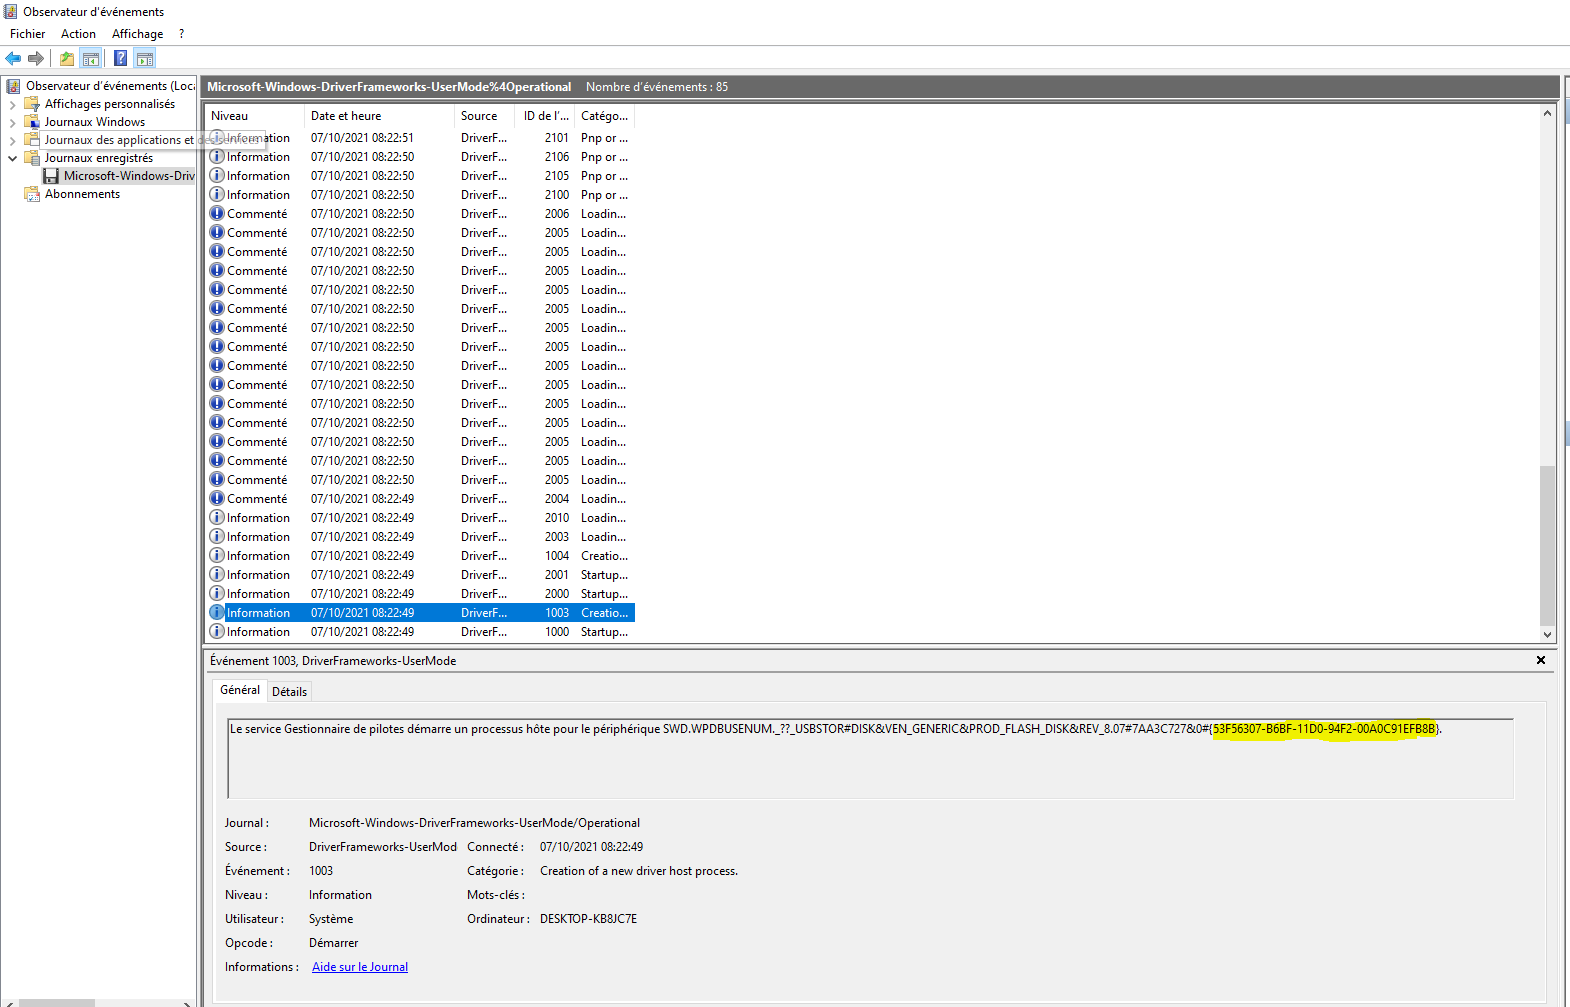
\includegraphics[width=17cm]{images/sameuuid.png}
    \caption{Logs de la clé USB}
    \label{fig:sameuuid}
\end{figure}







\newpage
\section{Analyse du disque du suspect}

Dans l'onglet OS Account de l'outil Autopsy, nous retrouvons le nom d'un compte utilisateur qui est le même que celui du suspect (\emph{voir figure \ref{fig:infos_user_suspect}} ).

\begin{figure}[H]
    \centering
    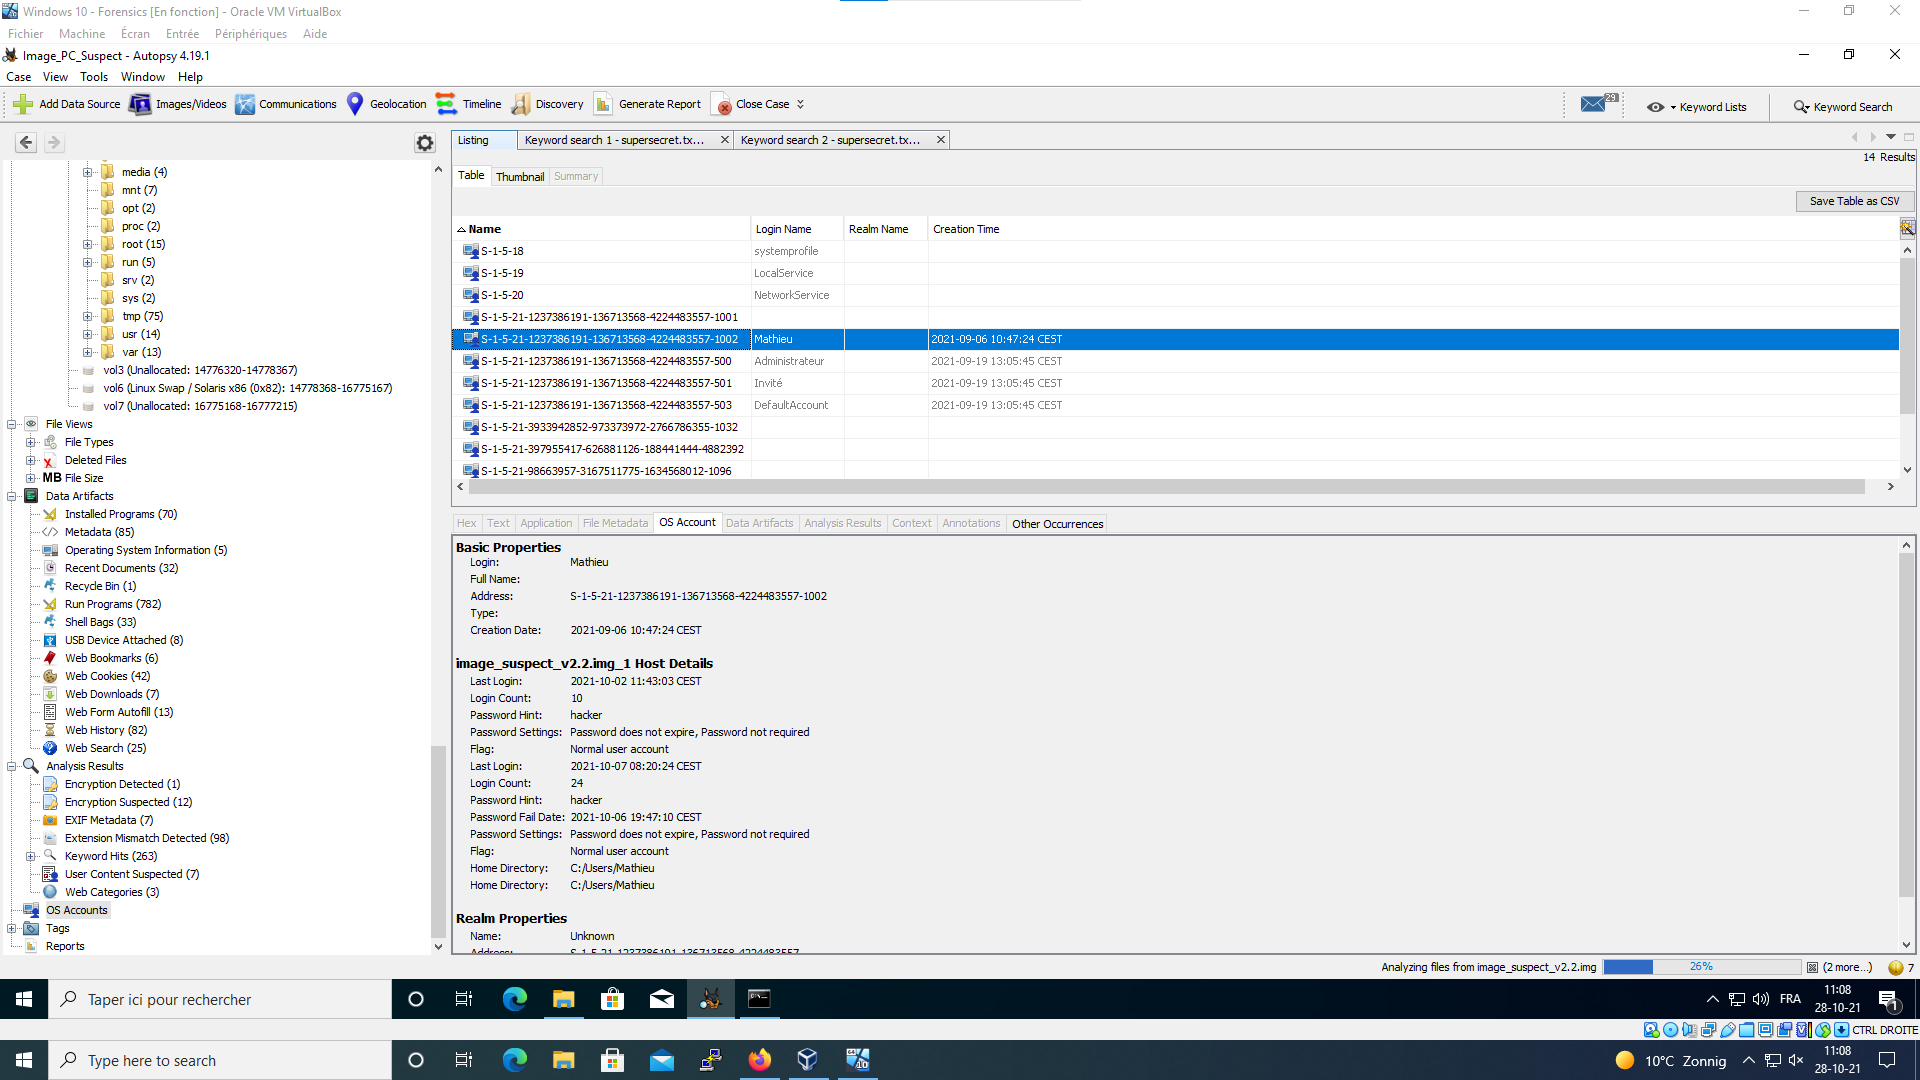
\includegraphics[width=17cm]{images/User_infos.png}
    \caption{Informations du compte utilisateur}
    \label{fig:infos_user_suspect}
\end{figure}

Nous commençons alors notre analyse en recherchant l'historique de recherche de l'utilisateur. Pour cela nous nous rendons à \emph{C{}:$\backslash$Users$\backslash$Mathieu$\backslash$Appdata$\backslash$Roaming$\backslash$Mozilla$\backslash$Firefox} et nous trouvons ainsi le dossier comportant toutes les données intéressantes liées au navigateur Firefox. Une fois le fichier de l'historique trouvé, nous pouvons constater plusieurs recherches en lien avec le CHR de Namur ainsi qu'avec le covid (\emph{voir figure \ref{fig:historique}})

\begin{figure}[H]
    \centering
    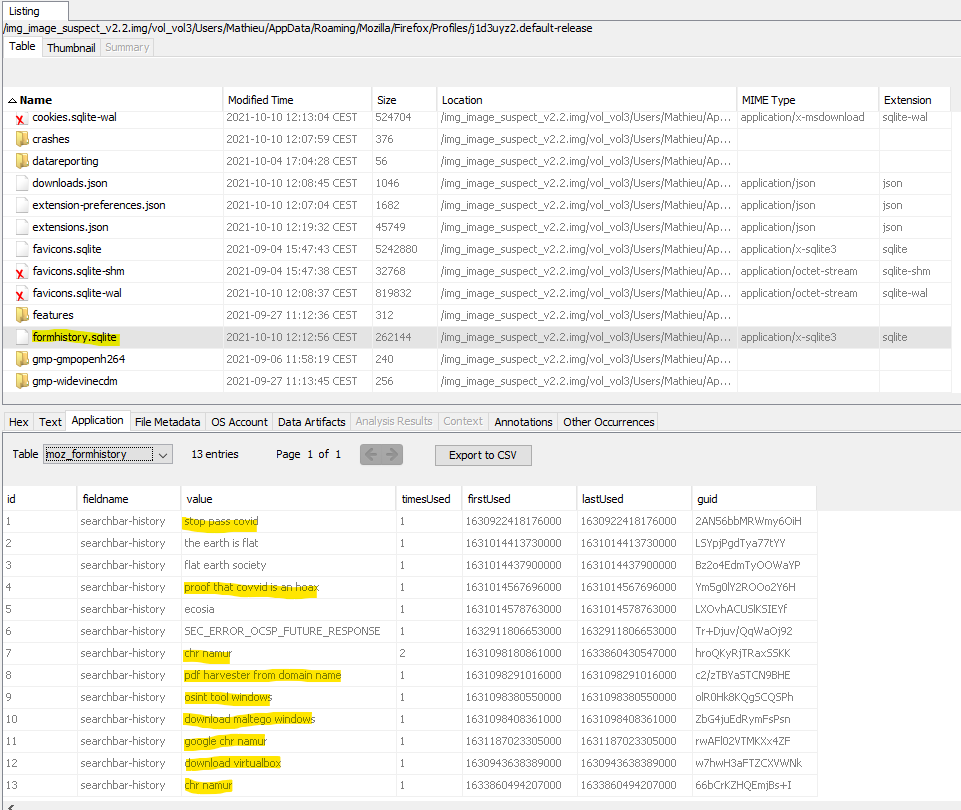
\includegraphics[width=14cm]{images/historique.png}
    \caption{Historique Firefox}
    \label{fig:historique}
\end{figure}

Dans l'onglet web bookmarks du logiciel Autopsy, tous les liens web ayant été utilisé en favoris dans le navigateur du suspect sont repris.\\
Sur la figure \ref{fig:lien_google_map}, on observe que l'un des liens correspond à un lien google map contenant des coordonnées et le nom du CHR de Namur.

\begin{figure}[H]
    \centering
    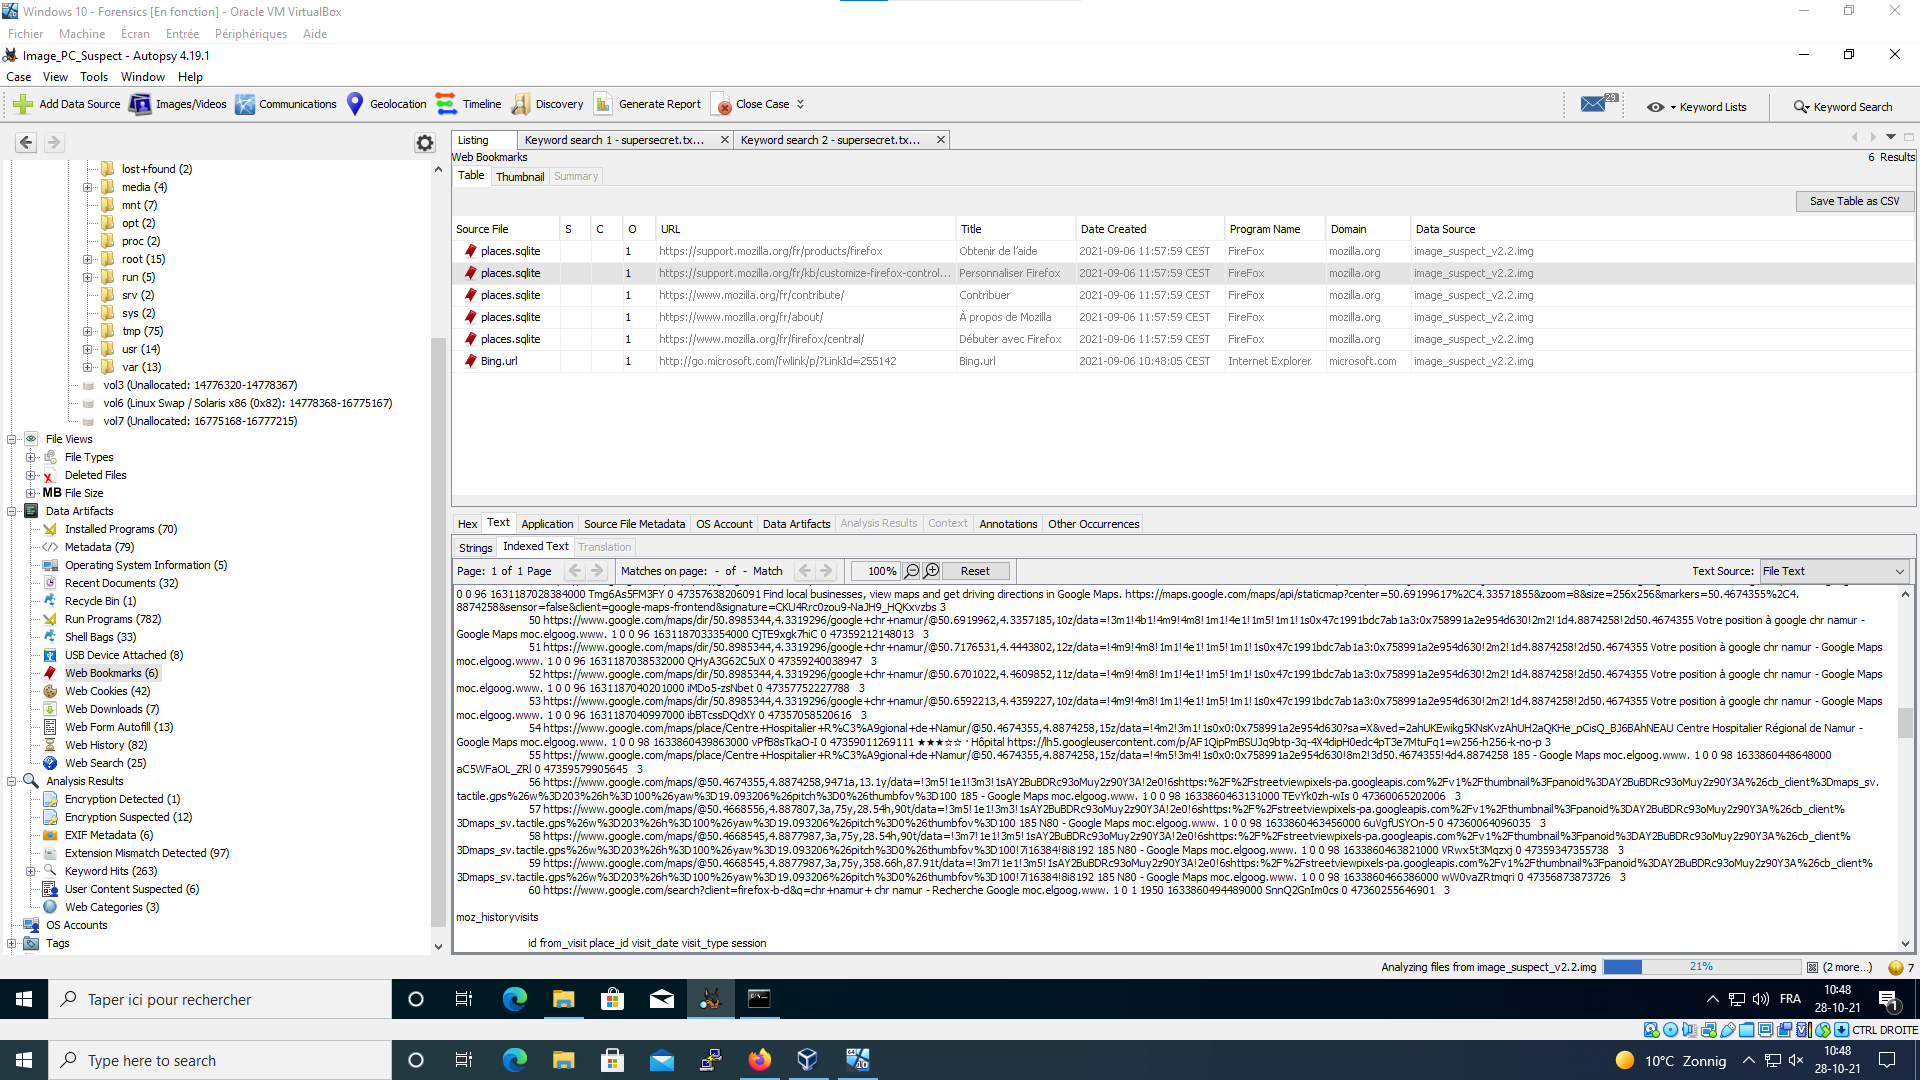
\includegraphics[width=14cm]{images/google_map_1.png}
    \caption{Lien google map trouvé dans l'onglet bookmarks d'Autopsy}
    \label{fig:lien_google_map}
\end{figure}

Si on utilise ce lien dans un navigateur web, on observe dans la figure 5 que celui-ci affiche un itinéraire sur google map.\\
Le lieu de départ correspond à un endroit proche de Bruxelles (\emph{voir figure \ref{fig:itinéraire_google_map}}). \\
Les hypothèses peuvent être que :
\begin{itemize}
    \item le suspect vit à cet endroit
    \item le suspect à utilisé cet endroit pour planifier son attaque
    \item le suspect à un complice qu'il devait rejoindre à cet endroit
\end{itemize}

\begin{figure}[H]
    \centering
    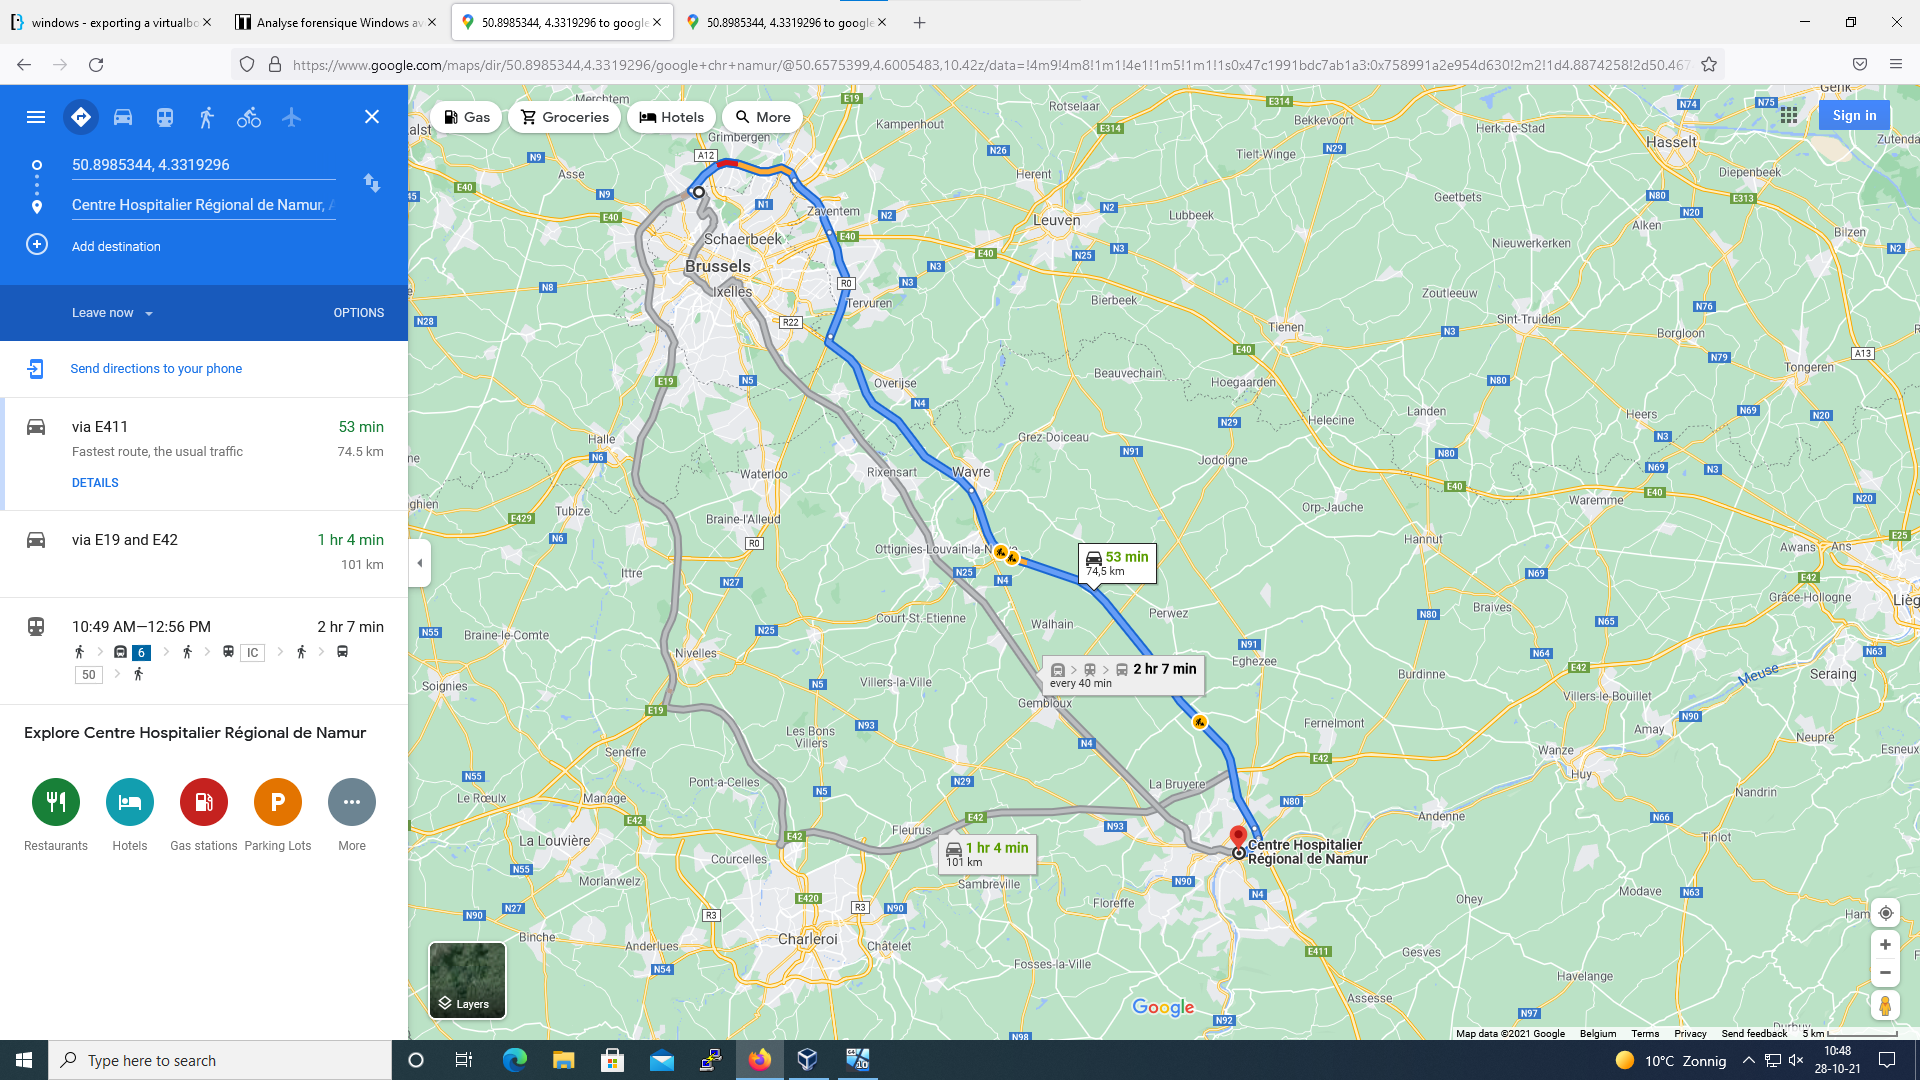
\includegraphics[width=13cm]{images/google_map_2.png}
    \caption{Itinéraire google map}
    \label{fig:itinéraire_google_map}
\end{figure}



Dans le dossier Downloads de l'utilisateur Mathieu, différents fichiers ont été trouvés (\emph{voir figure \ref{fig:Fichiers_suspects_downloads}} ) :
\begin{itemize}
    \item Un fichier \emph{"organisation\_medicale\_du\_chrn5.pdf"}, une preuve concernant l'intérêt que le suspect pouvait avoir pour le CHR.
    \item Une archive \emph{"virus.tar.gz"} considérée comme suspecte vu le nom qui lui est attribué. 
\end{itemize}

\begin{figure}[H]
    \centering
    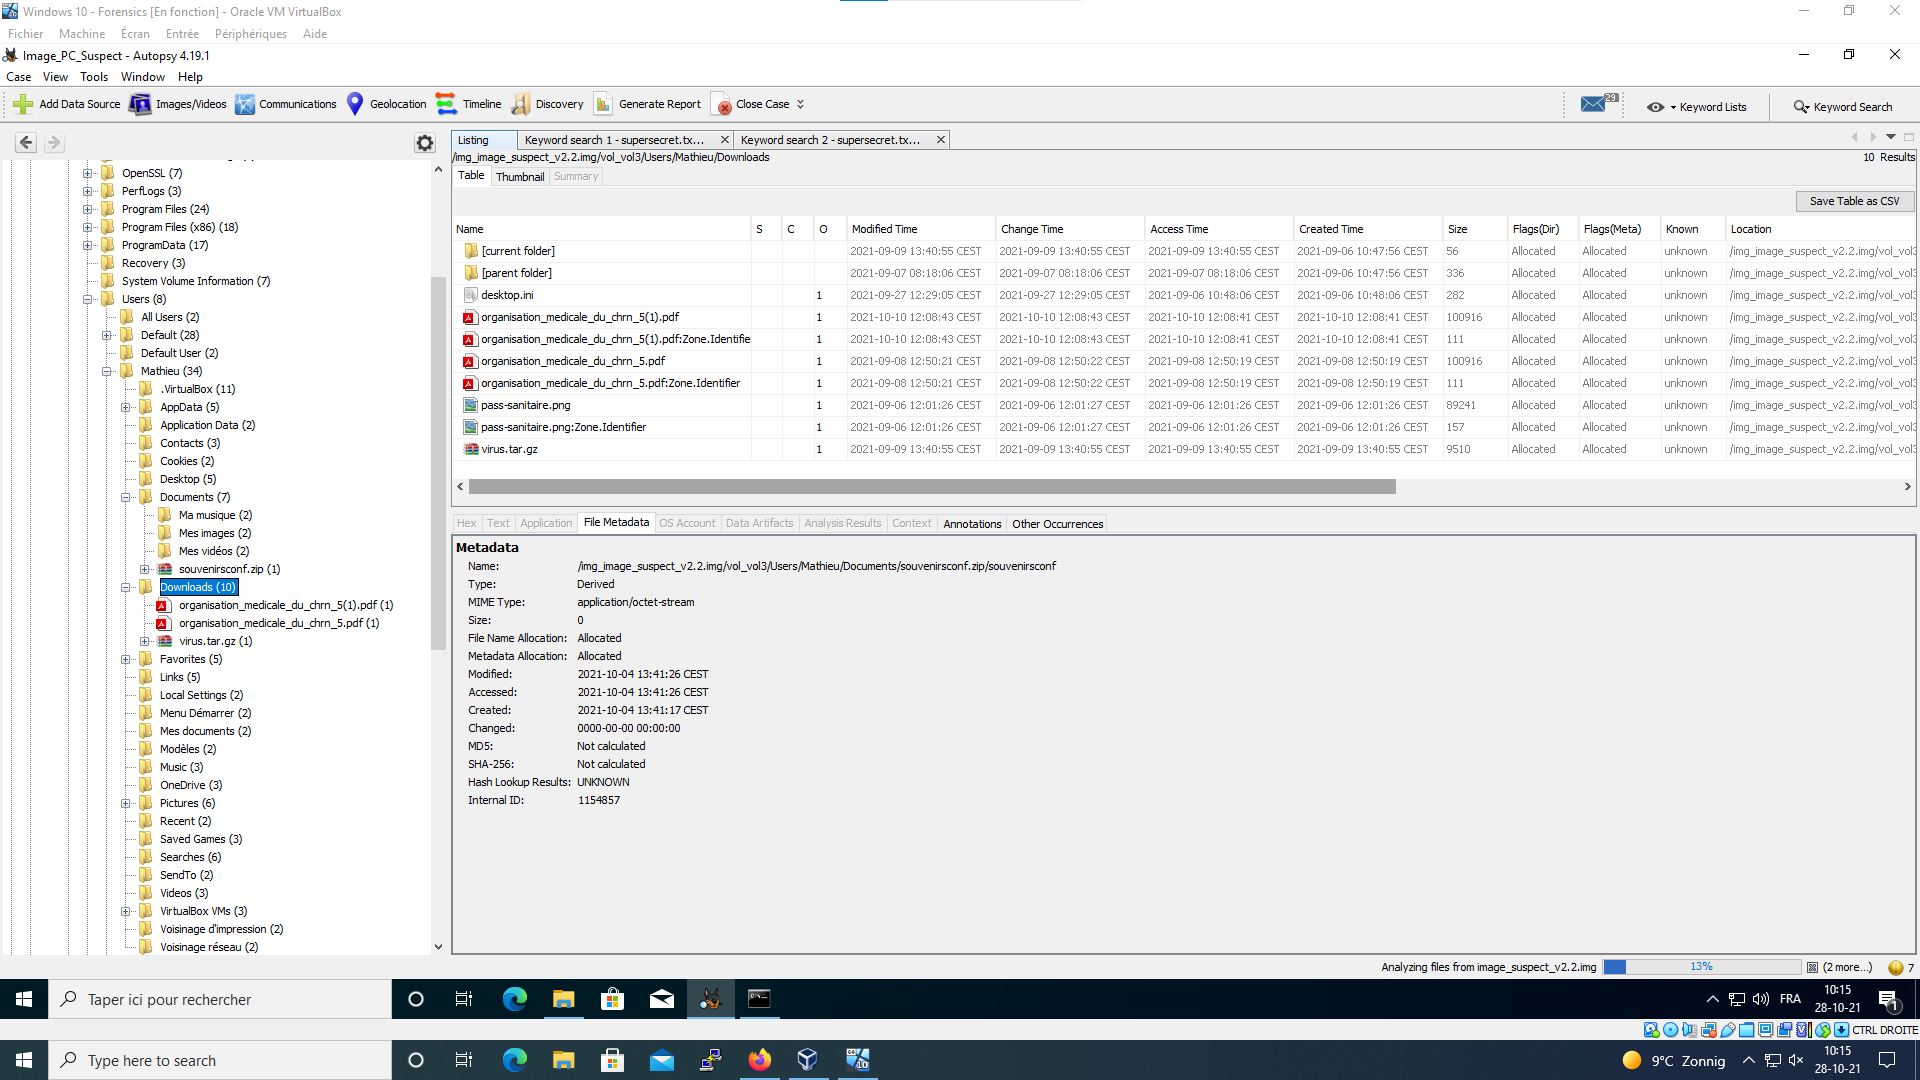
\includegraphics[width=14cm]{images/fichiers_dossier_downloads.png}
    \caption{Fichiers suspects dans le dossier Downloads}
    \label{fig:Fichiers_suspects_downloads}
\end{figure}

Dans le dossier Documents de l'utilisateur Mathieu, nous avons trouvé un fichier zip chiffré nommé souvenirsconf. Nous émettons l'idée qu'il s'agisse du dossier contenant les 4 images trouvées sur la clé USB lors de l'analyse précédente. Sur l'image de la figure \ref{fig:Fichier_souvenirsconf}, on observe d'ailleurs que dans ce fichier zip, il existe des dossiers auxquels nous ne pouvons pas accéder nommés \textbf{\textit{000X.JPG}} \\ \smallskip
Pour vérifier notre hypothèse, nous avons utilisé la méthode de bruteforce pour obtenir le mot de passe de l'archive. La méthode de bruteforce est utilisée pour déchiffrer un mot de passe en testant toutes les combinaisons possibles. Nous avons utilisé le programme \ref{code:bruteforce} (voir ci-dessous) et il s'est avéré que nos soupçons étaient exacts : il s'agit des 4 images retrouvées lors de la précédente analyse.

\begin{figure}[H]
    \centering
    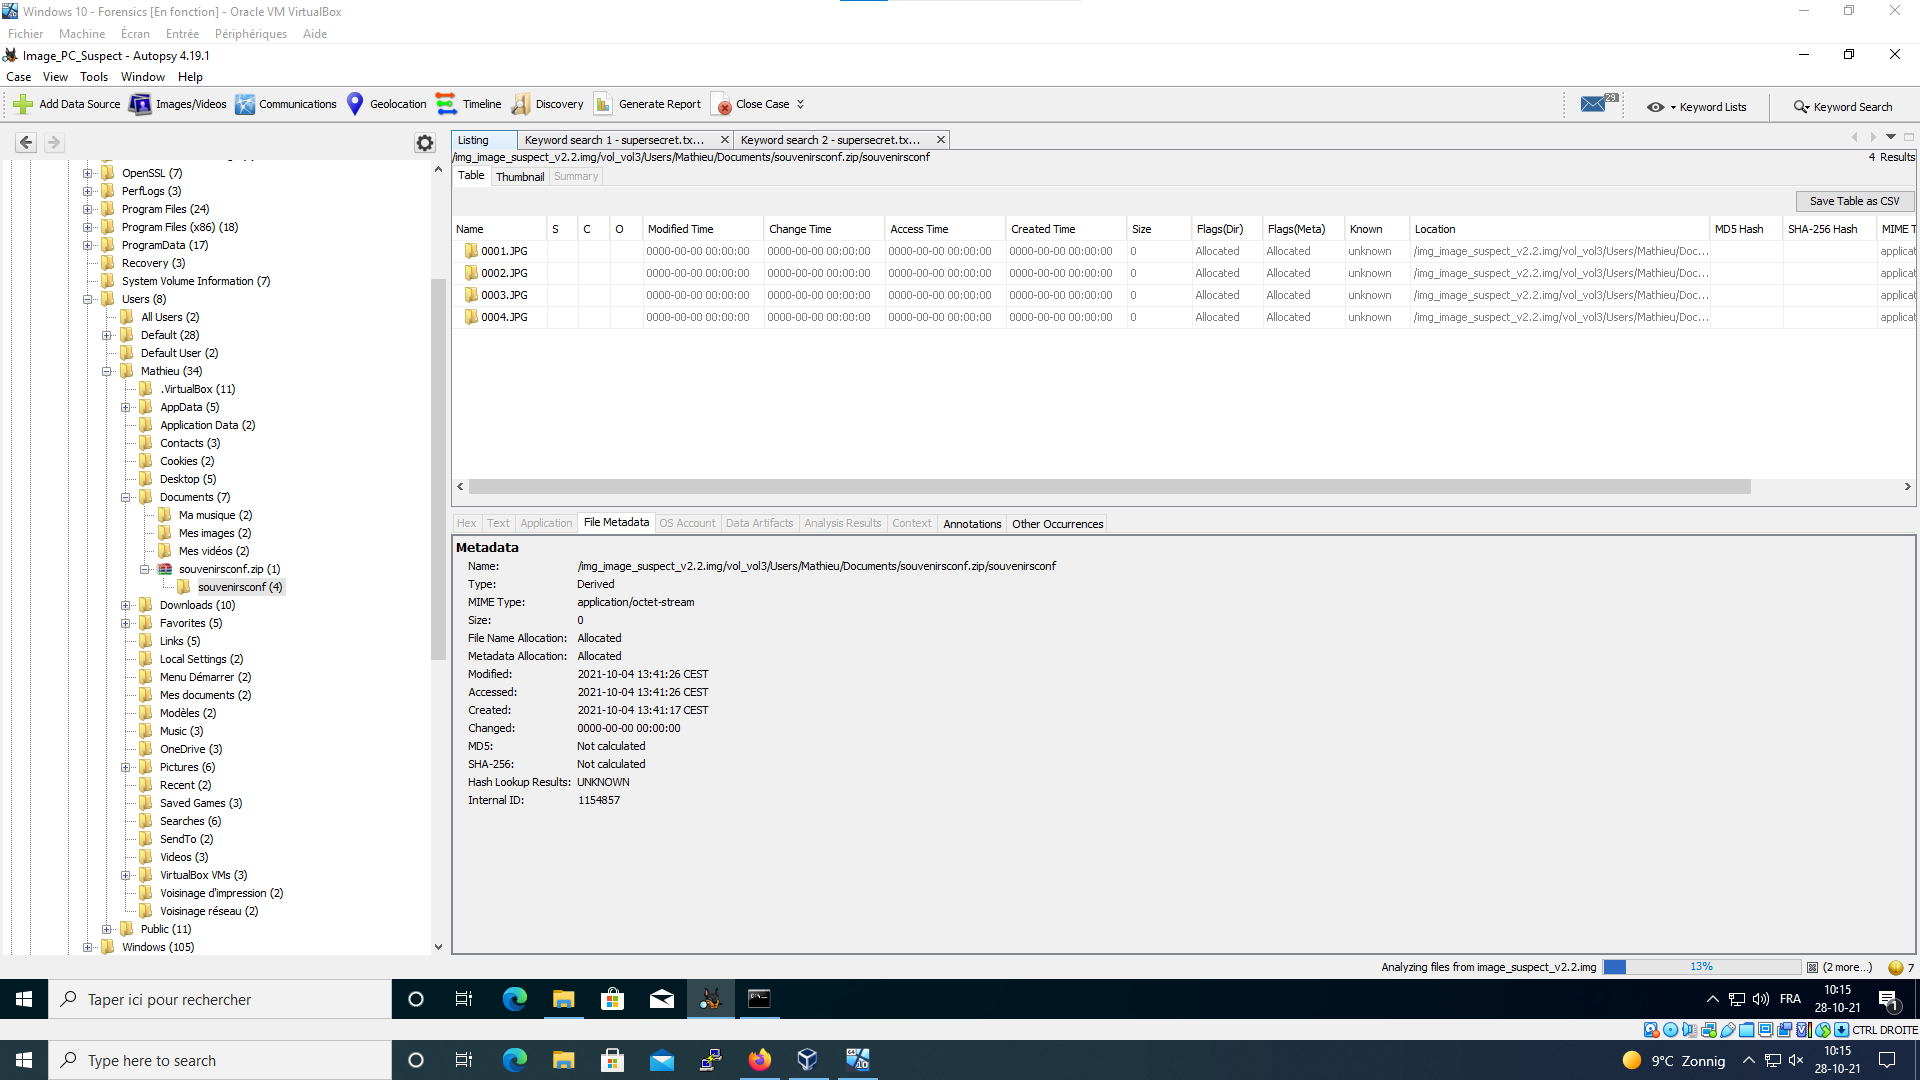
\includegraphics[width=15cm]{images/souvenirs.png}
    \caption{Fichier zip chiffré souvenirsconf}
    \label{fig:Fichier_souvenirsconf}
\end{figure}

\begin{code}\small
\begin{minted}[xleftmargin=20pt,linenos]{python}
import zipfile

def bruteforce_password(password_list, zip_file):
    obj = zipfile.ZipFile(zip_file)

    with open(password_list, 'rb') as file:
        for password in file:
            try:
                obj.extractall(pwd=password)
                print("Password is", password.decode())
                return
            except: pass

    print("Password not found")

password_list = "/usr/share/wordlists/rockyou.txt"
zip_file = "souvenirsconf.zip"

bruteforce_password(password_list, zip_file)
\end{minted}
\caption{Bruteforce de l'archive zip chiffrée}
\label{code:bruteforce}
\end{code}

Le logiciel Autopsy a pu retrouver différentes adresses e-mail dans l'image du disque. Et notamment des adresses d'employés du CHR. On observe d'ailleurs l'une de ces adresses sur la figure 8. Ces adresses ont peut-être permis au suspect de se procurer des informations sensibles pour planifier son attaque à l'aide de méthodes comme le phishing ou autres.

\begin{figure}[H]
    \centering
    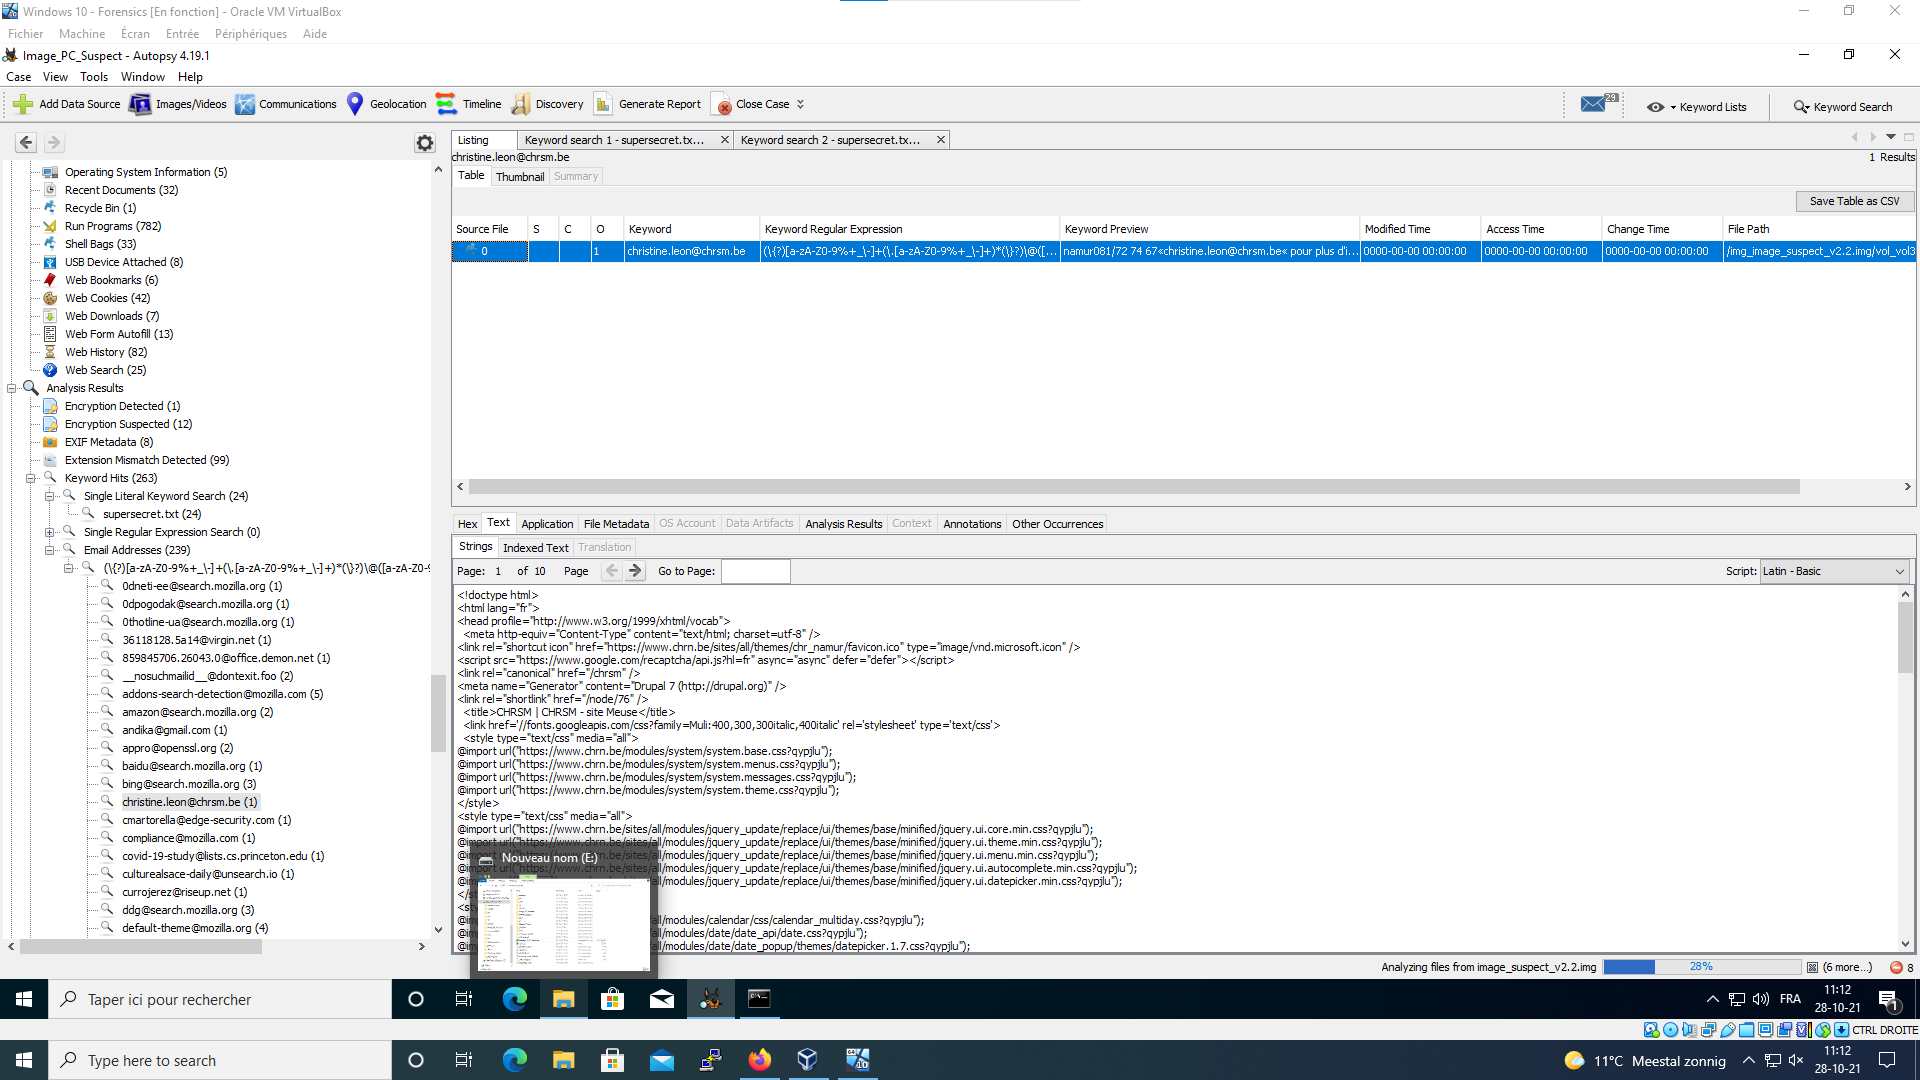
\includegraphics[width=15cm]{images/mail_chr.png}
    \caption{Adresses e-mail d'employé du CHR}
    \label{fig:mail-chr}
\end{figure}

Lors de l'analyse du disque, nous avons pu trouver un fichier vdi nommé AttackMachine (\emph{voir figure \ref{fig:linuxattack}} ). \\
Le format de fichier vdi est le format utilisé par VirtualBox lors de la création d'une machine virtuelle. Le fichier trouvé correspond donc au disque dur virtuel d'une machine virtuelle. Pour pouvoir utiliser ce fichier, il faut le convertir en une image au format raw (voir annexe \ref{sec:ConvertToRaw}). Le fichier pourra ensuite être analysé dans Autopsy afin de trouver de potentielles nouvelles preuves.

\begin{figure}[H]
    \centering
    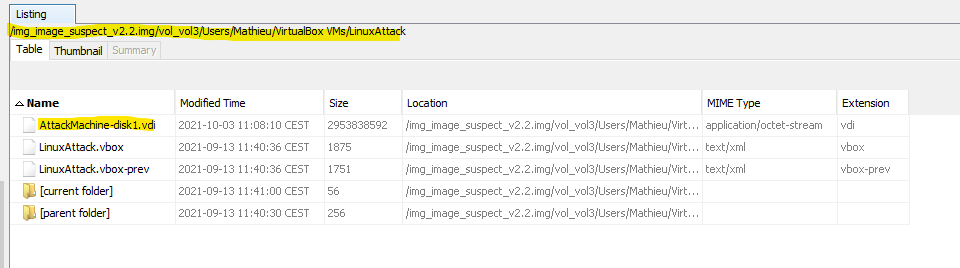
\includegraphics[width=15cm]{images/linuxattack.png}
    \caption{Disque dur virtuel trouvé}
    \label{fig:linuxattack}
\end{figure}

Sur l'ordinateur du suspect, nous avons aussi trouvé un lien venant de son historique de navigation (figure \ref{fig:LienSaintLuc}) menant à des informations sur l'hôpital Saint-Luc à Bouge (figure \ref{fig:fichierSaintLuc}). Nous émettons l'hypothèse que le suspect avait l'intention de s'en prendre à ce deuxième hôpital.

\begin{figure}[H]
    \centering
    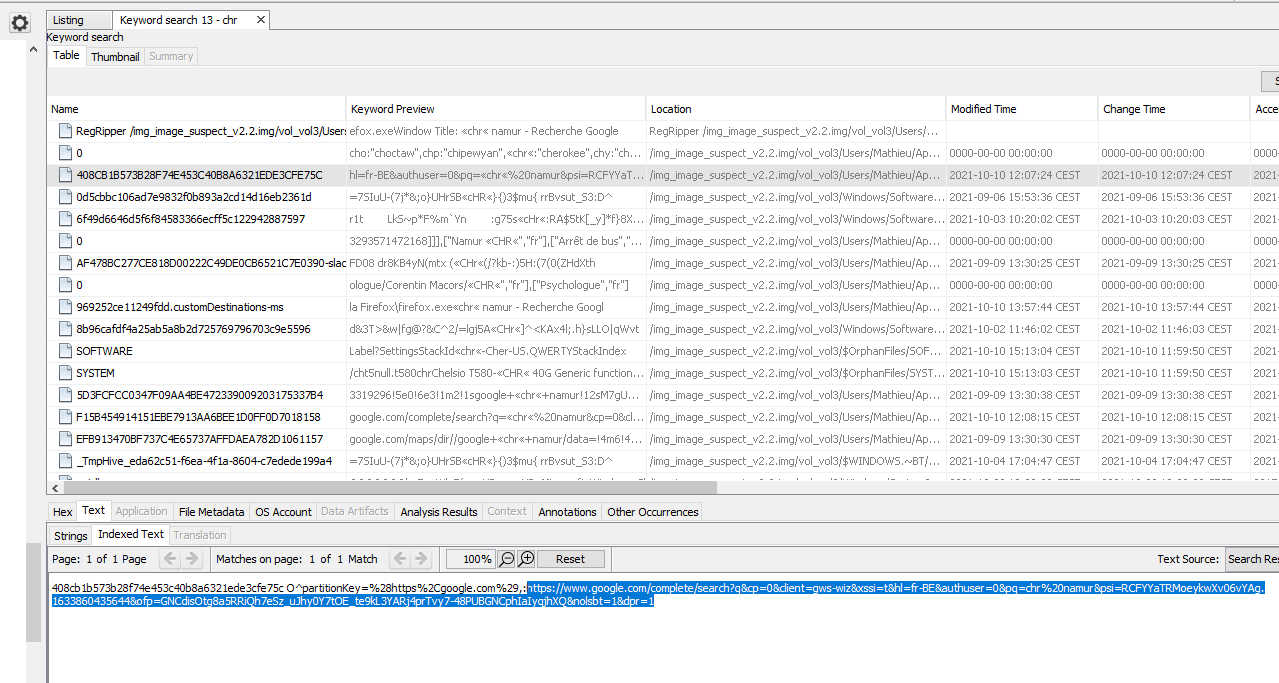
\includegraphics[width=0.99\linewidth]{images/Capture-009.PNG}
    \caption{Présence d'un lien menant à des données vers un deuxième hôpital dans l'historique du suspect}
    \label{fig:LienSaintLuc}
\end{figure}
\begin{figure}[H]
    \centering
    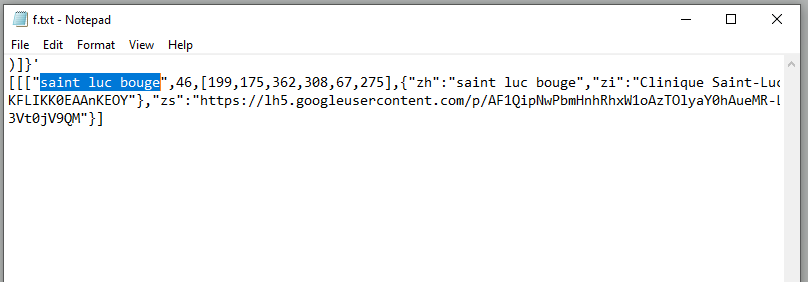
\includegraphics[width=14cm]{images/Capture-011.PNG}
    \caption{Informations sur un deuxième hôpital trouvées en suivant un lien dans l'historique du suspect}
    \label{fig:fichierSaintLuc}
\end{figure}










\newpage
\section{Analyse du disque virtuel trouvé}

L'analyse du disque de la machine virtuelle sur Autopsy à permis de trouver un dossier "Python-Backdoor-master" dans le quel on peut retrouver un dossier "old\_Keylogger" avec un fichier "source.py" à l'intérieur. Ce fichier correspond au code python d'un keylogger. 
Un keylogger est un malware installé sur une machine cible servant à enregistrer les frappes faites au clavier par l'utilisateur. Ce fichier pourrait potentiellement avoir été utilisé par le suspect pour obtenir des informations sensibles sur le CHR.

\begin{figure}[H]
    \centering
    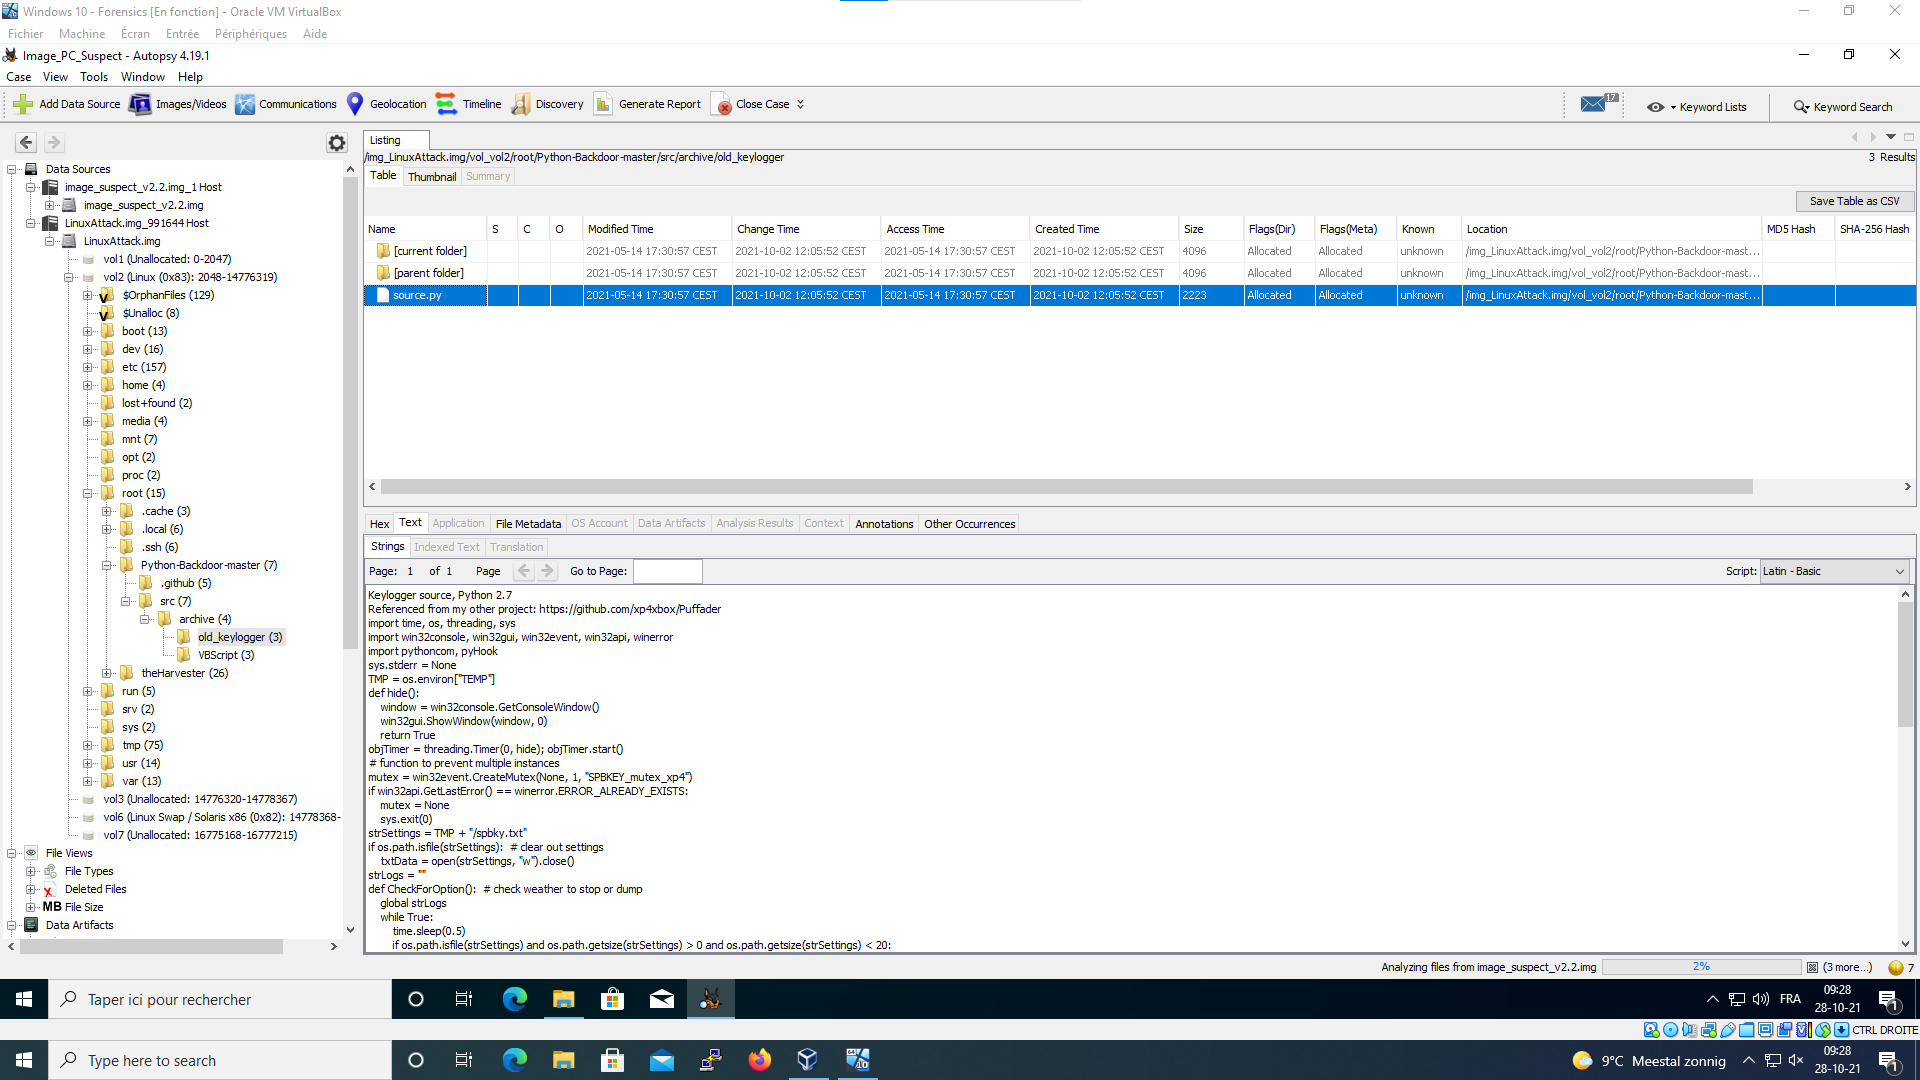
\includegraphics[width=14cm]{images/oldkeylogger.png}
    \caption{Fichier source d'un keylogger}
    \label{fig:keylogger}
\end{figure}

Dans ce dossier Python Backdoor, un autre dossier s'y trouve nommé VBScript. À l'intérieur se trouve le fichier "Disable Task Manager.vbs". VBScript est un langage de scripting pouvant être exécuté sous Windows et l'extension vbs est celle qui correspond à ce langage. Nous pensons que ce script pourrait servir à désactiver le task manager d'un ordinateur. Peut-être dans le but d'empêcher les utilisateurs ou administrateurs d'accéder à certaines informations.

\begin{figure}[H]
    \centering
    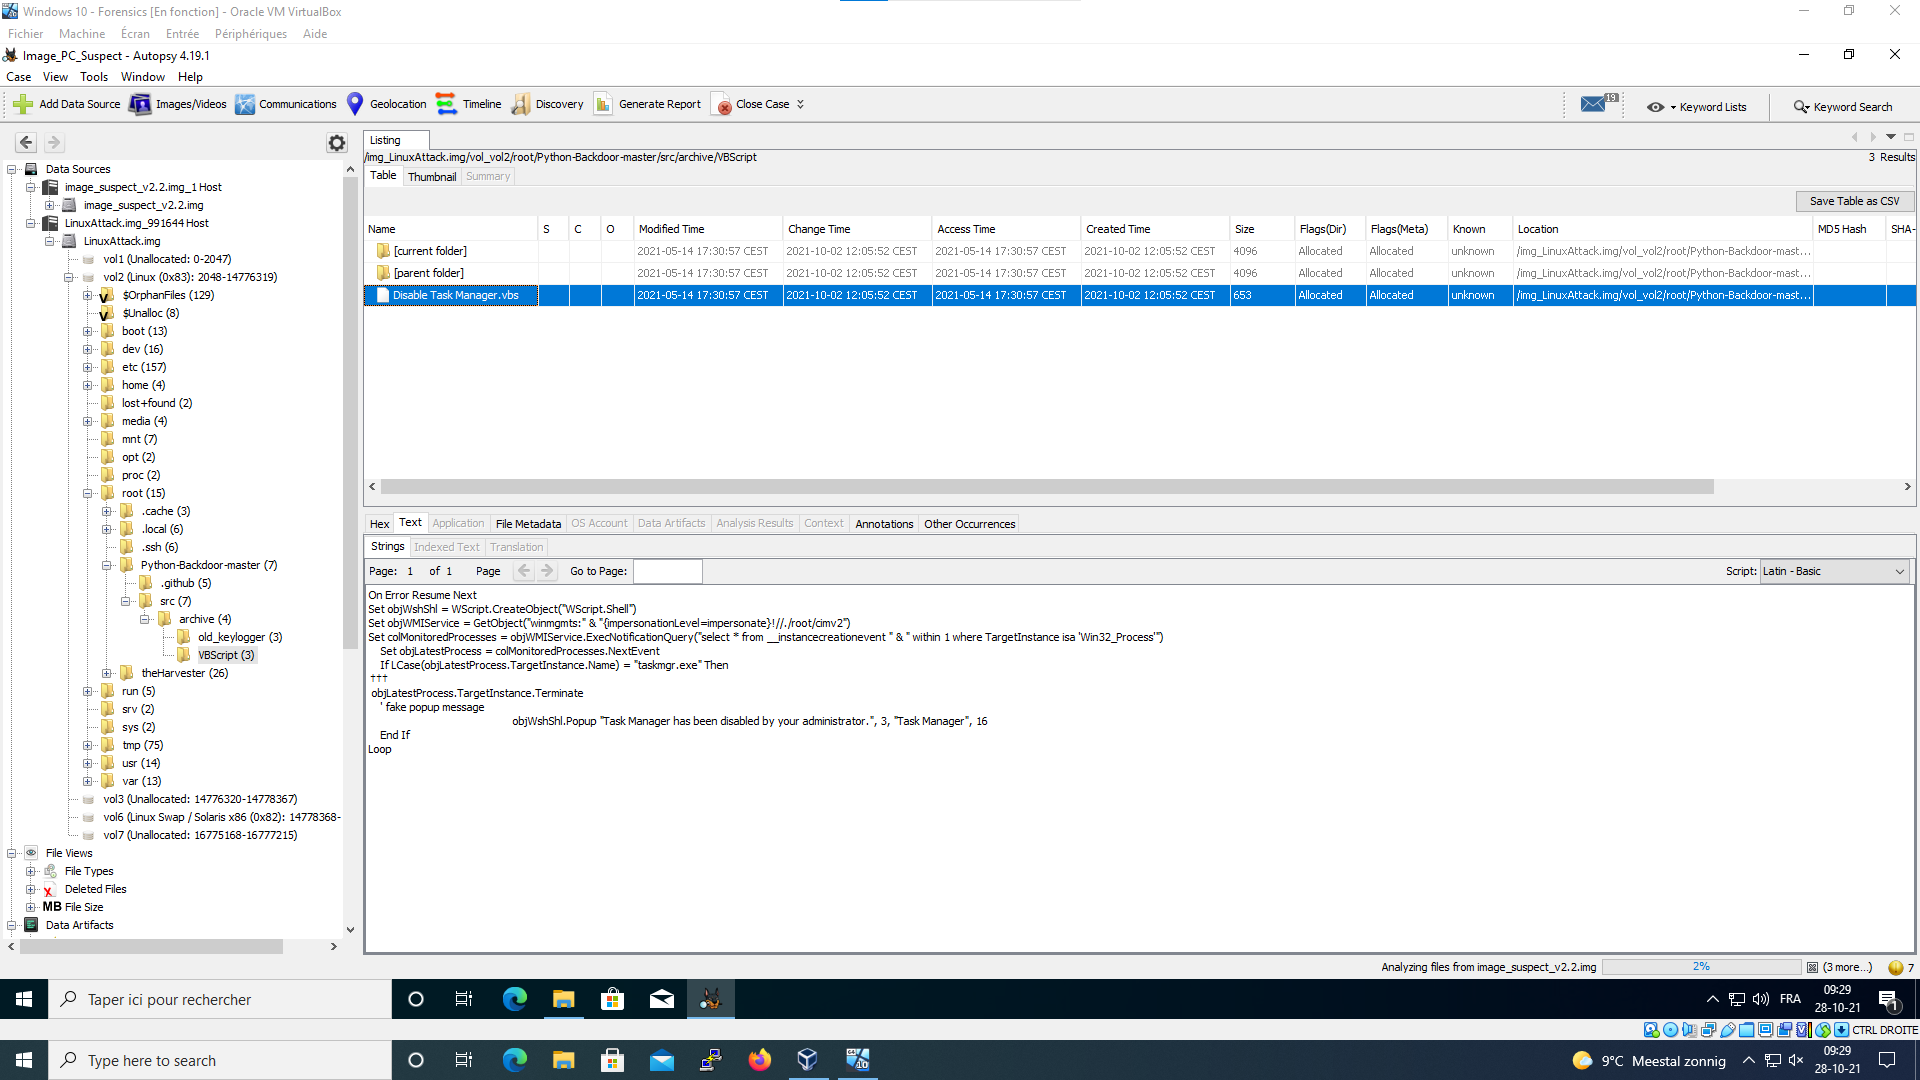
\includegraphics[width=14cm]{images/VBScript.png}
    \caption{Fichier vbs}
    \label{fig:VBS}
\end{figure}










\newpage
\section{Analyse de l'archive "virus.tar.gz"}

Lorsque l'on décompresse le fichier \emph{"virus.tar.gz"}, nous obtenons 2 fichiers binaires exécutable :
\begin{itemize}
    \item \emph{bad}
    \item \emph{server}
\end{itemize}

Dans un environnement contrôlé, nous commençons par analyser le fichier \emph{server}. Pour cela, nous le lançons et obtenons ceci :

\begin{figure}[H]
    \centering
    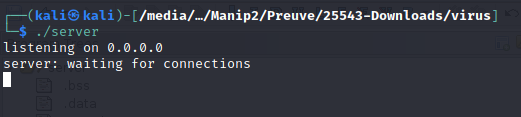
\includegraphics[width=13cm]{images/server.png}
    \caption{Lancement du fichier "server"}
    \label{fig:Fichier_server}
\end{figure}

Nous pouvons constater que celui-ci attend vraisemblablement la connexion d'un client. Nous pouvons donc imaginer qu'il s'agit du fichier "bad" que nous analyserons par la suite.\\
Ensuite, nous le décompilons et le désassemblons grâce à l'outil Ghidra (version 9.1). Sur la \emph{Figure \ref{fig:ghidra_server}}, nous pouvons voir la fonction main. Nous constatons donc que celui-ci ouvre bien un socket (\emph{voir annexe \ref{sec:def_socket}}) et qu'il écrit les données reçues dans un fichier mis en argument au programme.

\begin{figure}[H]
    \centering
    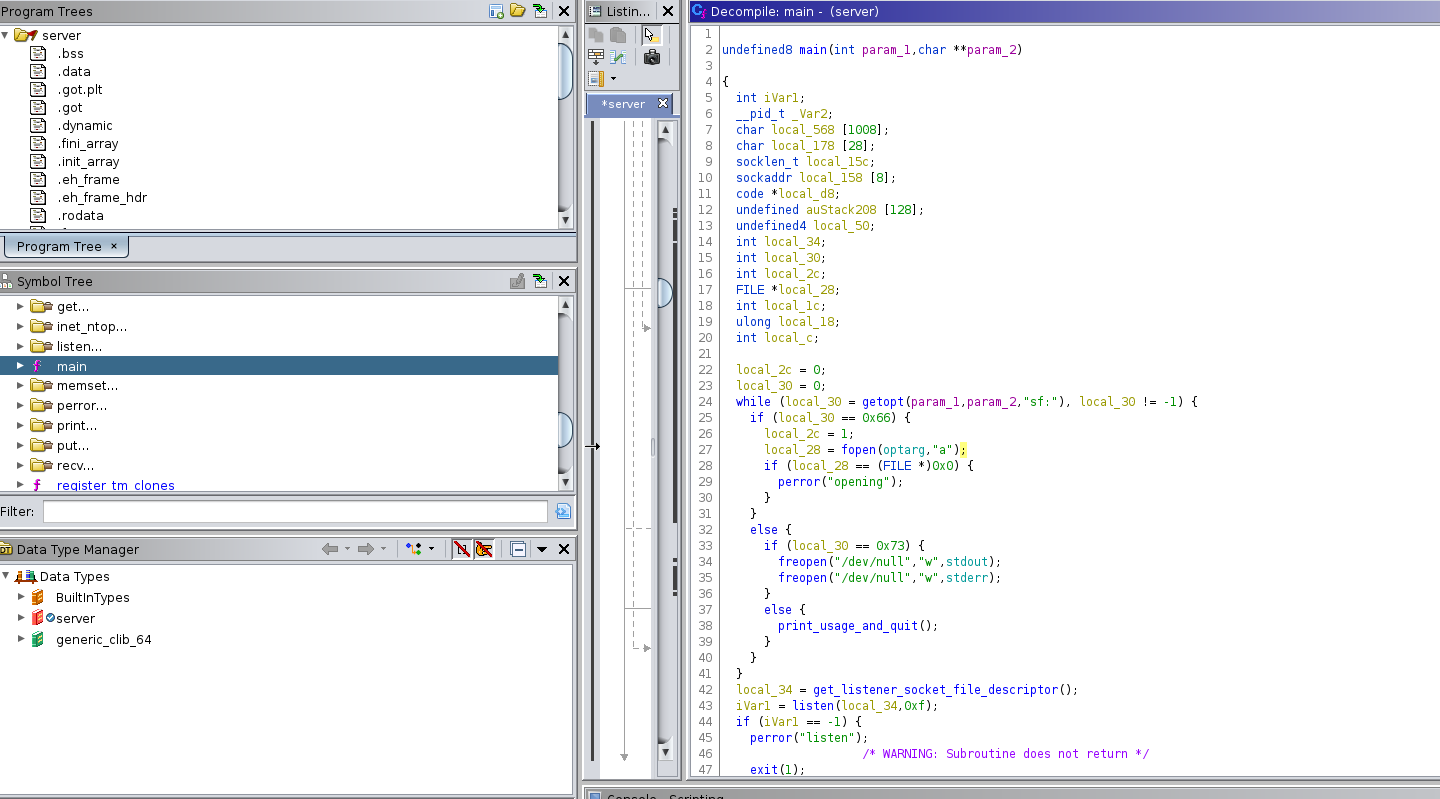
\includegraphics[width=16cm]{images/ghidraserver.png}
    \caption{Fonction main de l'exécutable "server"}
    \label{fig:ghidra_server}
\end{figure}

Nous passons maintenant au fichier "bad". Étant donné que nous n'avons aucun résultat lorsque l'on essaie de le lancer, nous passons directement à la phase de décompilation avec le même outil (Ghidra 9.1). Sur la \emph{Figure \ref{fig:ghidra_bad}}, nous retrouvons la fonction main. Pour résumer, nous constatons qu'il s'agit d'un keylogger (\emph{voir annexe \ref{sec:def_keylogger}}) qui essaie de se connecter à un socket.

\begin{figure}[H]
    \centering
    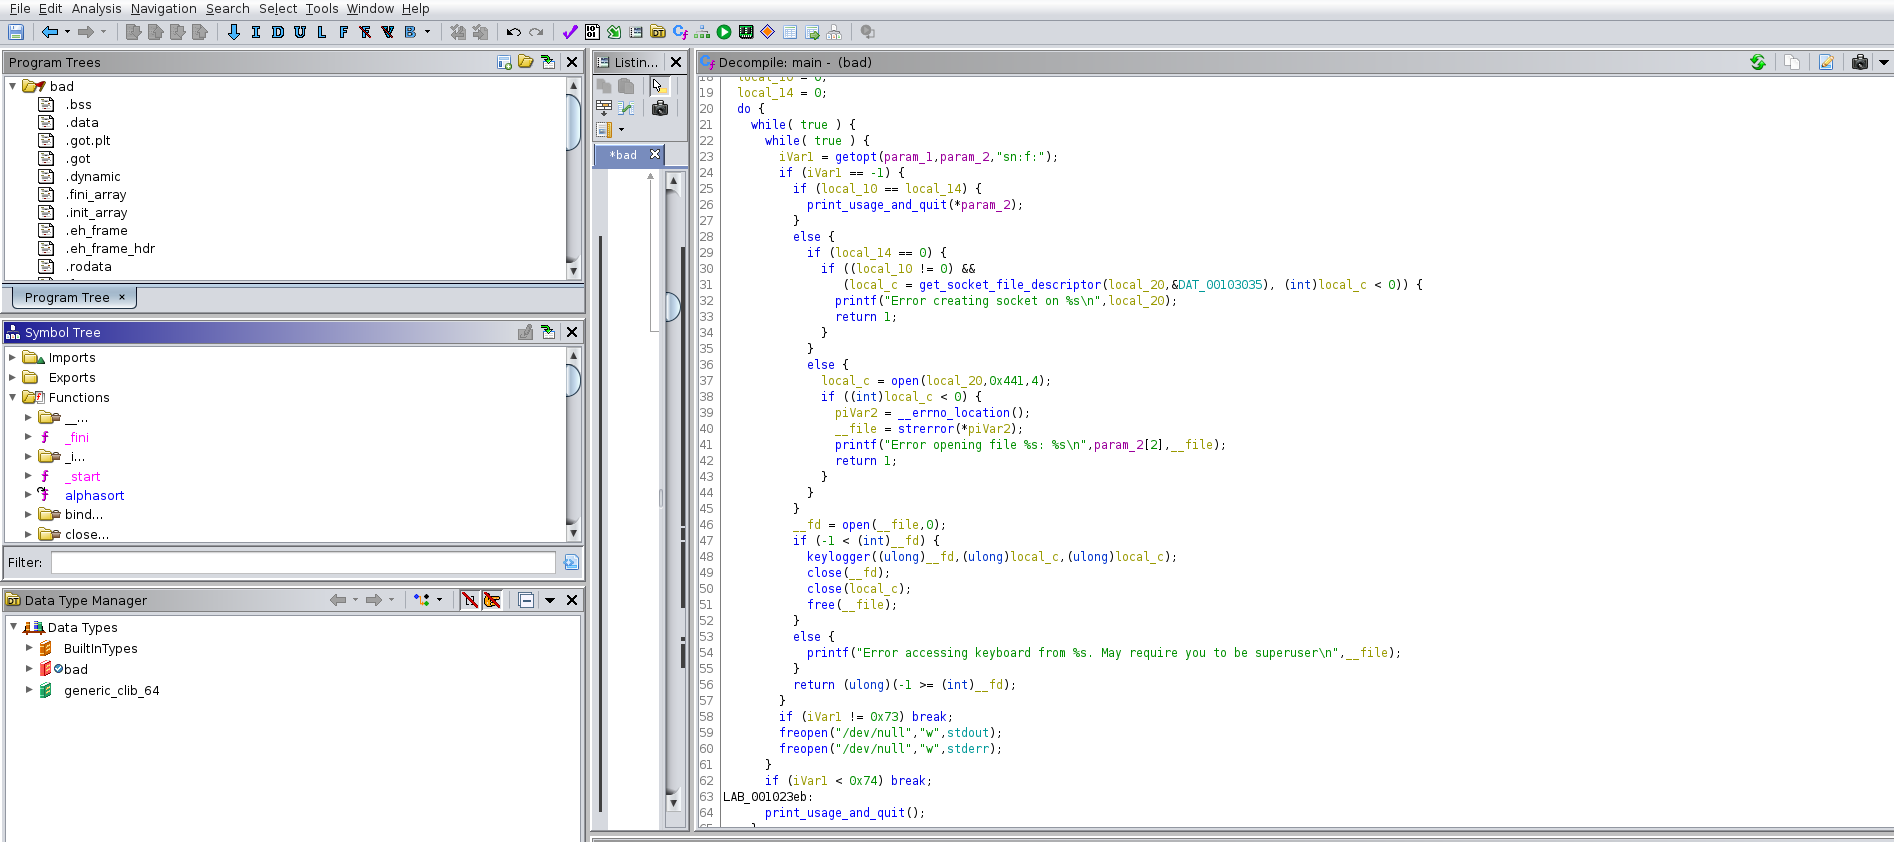
\includegraphics[width=16cm]{images/ghidrabad.png}
    \caption{Fonction main de l'exécutable "bad"}
    \label{fig:ghidra_bad}
\end{figure}

Pour résumer, le fichier "bad" est le malware qui envoie ses données au socket du programme "server" qui lui écrira toutes les données reçues dans un fichier mis en argument.









\section{Conclusion}
%%
Tout d'abord, nous avons pu établir et prouver le lien entre l'ordinateur du suspect et la clé retrouvée au CHR de namur, et ce grâce aux logs et à l'UUID de celle-ci. Ensuite, nous avons pu détailler son intérêt pour le CHR mais également, semblerait-il, pour d'autres établissements hospitaliers. Enfin, nous avons pu découvrir certains des outils utilisés pour mettre en place son attaque et la réaliser. Citons par exemple Maltego, TheHarvester, ou encore un keylogger.









\newpage \appendix










\section{Capture de la mémoire non-volatile et analyse de fichiers supprimés}



\subsection{Windows 10 - NTFS} \label{sec:CaptureWindows10}

Pour la capture de la mémoire non-volatile sur Windows, nous avons utilisé l'outil FTK Imager (version 4.5.0.3). En allant dans \textit{File} puis \textit{Create Disk Image} et en sélectionnant l'option \textit{Physical Drive}, on peut créer l'image du disque que l'on souhaite (figure \ref{fig:001ftk}).

\begin{figure}[H]
    \centering
    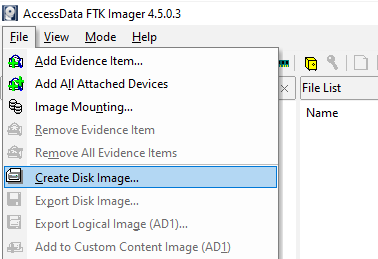
\includegraphics[width=8cm]{images/001-ftk-imager.PNG}
    \caption{Commencement d'une nouvelle capture de la mémoire non-volatile dans FTK Imager}
    \label{fig:001ftk}
\end{figure}

À l'aide du logiciel FTK Imager, il est aussi possible de récupérer certains fichiers supprimés. Sur la figure \ref{fig:002ftk}, vous pouvez voir les fichiers supprimés dans la corbeille. Et sur la figure \ref{fig:003ftk}, on voit les mêmes fichiers après avoir vidé la corbeille. Nous avons pu les récupérer parce que de nouvelles données n'ont pas été réécrites par-dessus, cependant, il est possible de perdre des informations une fois les fichiers supprimés.

\begin{figure}[H]
    \centering
    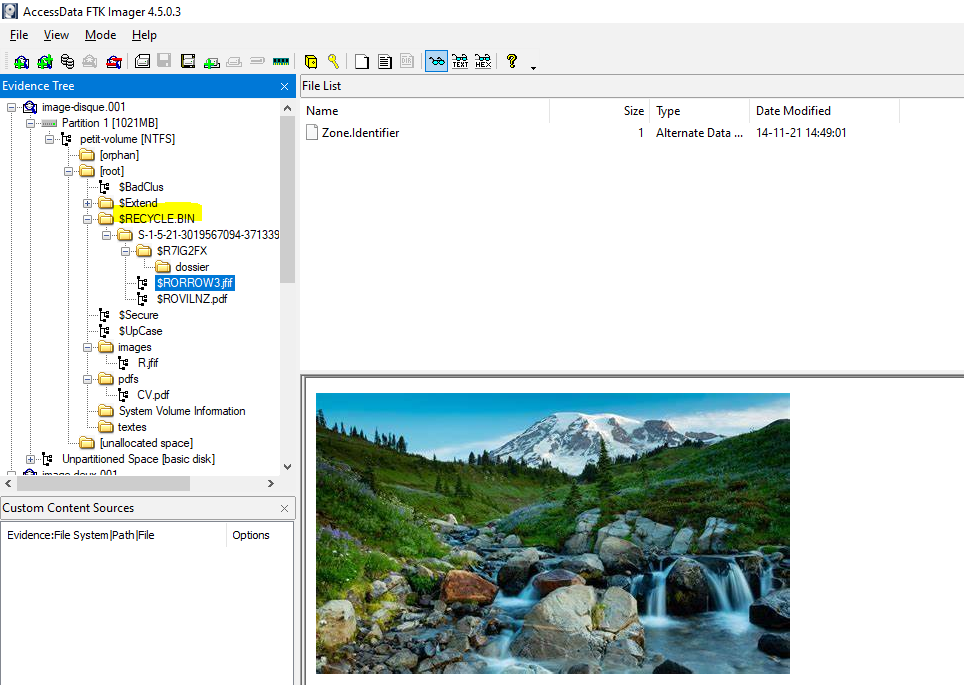
\includegraphics[width=15cm]{images/002-ftk-imager.PNG}
    \caption{Visualisation de fichiers dans la corbeille avec FTK Imager}
    \label{fig:002ftk}
\end{figure}
\begin{figure}[H]
    \centering
    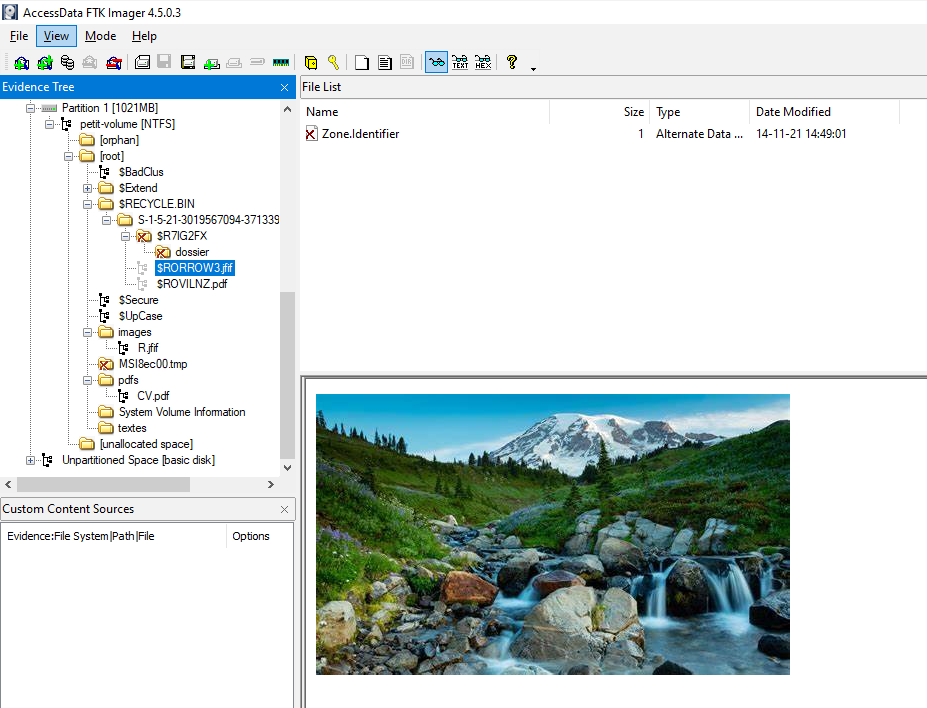
\includegraphics[width=15cm]{images/003-ftk-imager.PNG}
    \caption{Visualisation de fichiers supprimés après avoir vider la corbeille avec FTK Imager}
    \label{fig:003ftk}
\end{figure}

Pour analyser le fichier, on peut aussi utiliser le logiciel Autopsy (version 4.19.2) comme sur la figure \ref{fig:004ftk}. Sur cette capture, on voit plusieurs fichiers mis en évidence mais ils correspondent bien à un seul fichier. Le premier contient les données du fichier, le deuxième est un flux alternatif lié au fichier \cite{5} et le troisième contient le chemin du fichier dans le système de fichiers (dans ce cas: {\small \texttt{E:$\backslash$images$\backslash$OIP.jfif}}).

\begin{figure}[H]
    \centering
    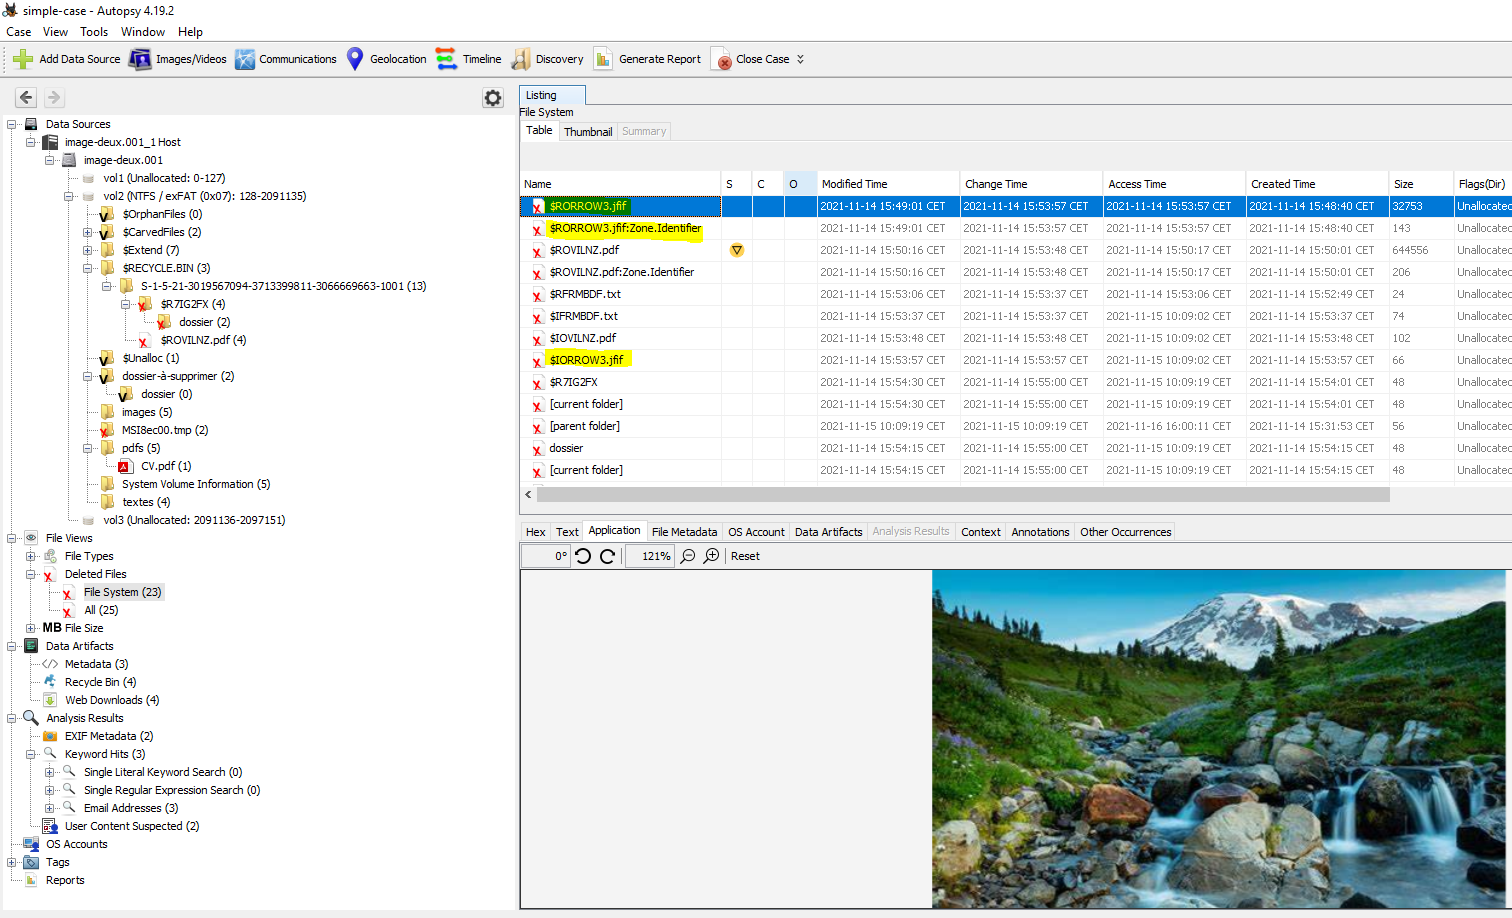
\includegraphics[width=0.99\linewidth]{images/004-ftk-imager.PNG}
    \caption{Visualisation de fichiers supprimés après avoir vidé la corbeille avec Autopsy}
    \label{fig:004ftk}
\end{figure}



\subsection{Linux - Ext4} \label{sec:CaptureLinux}

Pour la capture de la mémoire non volatile sur Linux, nous avons utilisé l'outil Guymager version 0.8.13. Il suffit de faire un clic droit sur le disque dont on veut faire une image, puis cliquer sur \textit{Acquire image} (figure \ref{fig:005ftk}).

\begin{figure}[H]
    \centering
    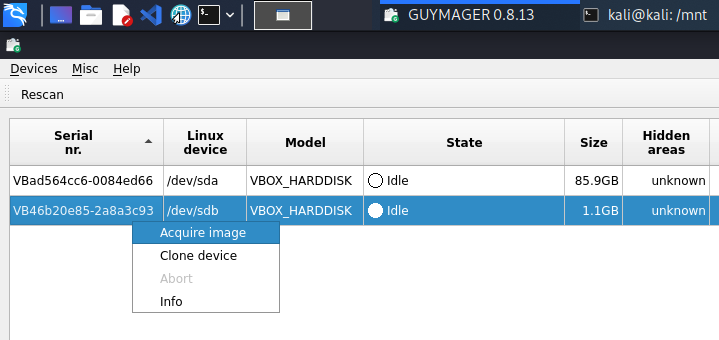
\includegraphics[width=0.75\linewidth]{images/005-guymager.PNG}
    \caption{Commencement d'une nouvelle capture de la mémoire non-volatile dans Guymager}
    \label{fig:005ftk}
\end{figure}

En analysant cette image comme vous pouvez le voir sur la figure \ref{fig:006ftk}, on retrouve les fichiers supprimés.

\begin{figure}[H]
    \centering
    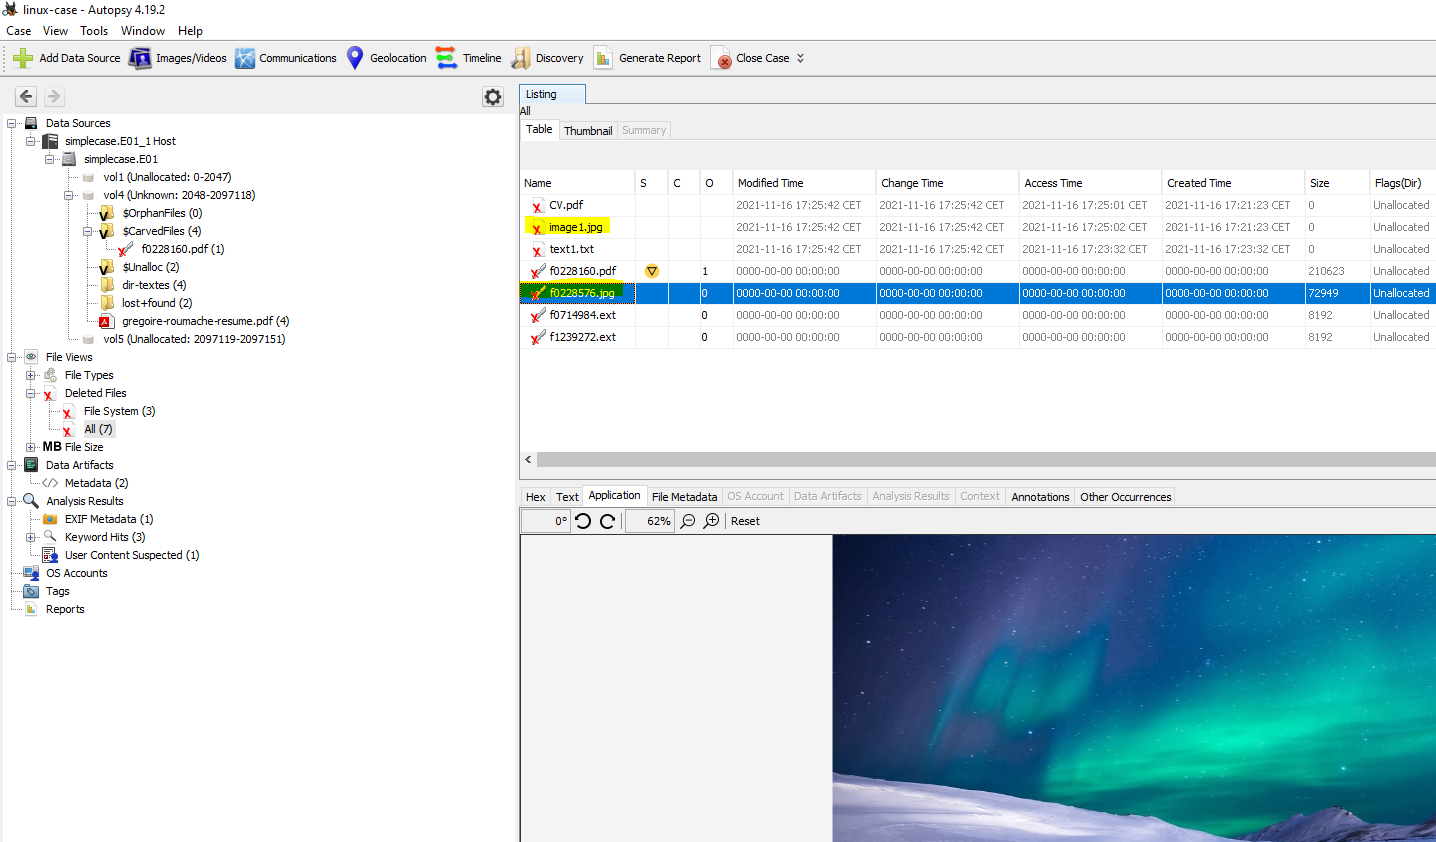
\includegraphics[width=0.99\linewidth]{images/006-autopsy.PNG}
    \caption{Visualisation de fichiers supprimés du système ext4 avec Autopsy}
    \label{fig:006ftk}
\end{figure}



\subsection{Comment placer une partition en read-only sur Windows et Linux}

Sur Windows, on peut utiliser les commandes suivantes \cite{1}: 
\begin{enumerate}
    \item {\small \texttt{diskpart}}, lance l'outil de gestion des partitions de Windows
    \item {\small \texttt{list volume}}, liste les partitions
    \item {\small \texttt{select volume <numéro>}}, sélectionne le volume
    \item {\small \texttt{attributes volume set readonly}}
\end{enumerate}

Sur Linux, on utilise la commande {\small \texttt{mount}} avec l'argument {\small \texttt{-o}} servant à préciser des options, suivi de {\small \texttt{"ro"}} pour read-only.









\section{Comment convertir un disque virtuel .vdi en image raw}\label{sec:ConvertToRaw}
Manipulation faite sur Windows 10 \cite{6}:
\begin{enumerate}
    \item Installer VirtualBox (si ce n'est pas déjà fait)
    \item Ouvrir une invite de commande
    \item Se diriger vers le dossier de VirtualBox \\
    (généralement \emph{C{}:$\backslash$Program Files$\backslash$Oracle$\backslash$VirtualBox})
    
    \item Utiliser l'outil VBoxManage.exe avec les arguments suivant (ref. \emph{Figure \ref{fig:vditoraw}}) :
    \begin{enumerate}
        \item "clonehd"
        \item Le fichier .vdi
        \item Le fichier de sortie
        \item "--format raw"
    \end{enumerate}
\end{enumerate}
\begin{figure}[H]
    \centering
    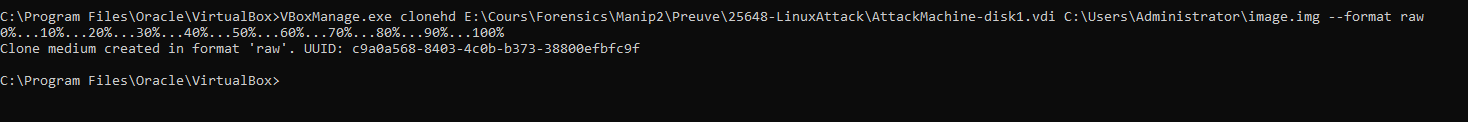
\includegraphics[width=1 \linewidth]{images/vditoraw.png}
    \caption{Commande pour convertir un disque virtuel (.vdi) en image raw}
    \label{fig:vditoraw}
\end{figure}









\section{Définition d'un socket} \label{sec:def_socket}
Un socket est connu comme un type de logiciel qui agit comme un point d'extrémité qui fonctionne en établissant une liaison de communication réseau bidirectionnelle entre l'extrémité du serveur et le programme de réception du client. On l'appelle aussi souvent un point d'aboutissement dans un canal de communication bidirectionnel. Un socket est capable de simplifier le fonctionnement d'un programme car les programmeurs n'ont plus qu'à se soucier de manipuler les fonctions du socket, ce qui leur permet de compter sur le système d'exploitation pour transporter correctement les messages sur le réseau. (ref. \cite{7})









\section{Définition d'un keylogger} \label{sec:def_keylogger}
Un keylogger est un " enregistreur de touche ". Autrement dit, c'est un spyware capable de détecter les frappes sur le clavier de votre ordinateur et de les mémoriser. Le tout, sans que vous le sachiez. Il permet donc à des cybercriminels de mettre à jour vos identifiants et codes d'accès sur vos comptes privés ou professionnels. (ref. \cite{8})








\newpage \addcontentsline{toc}{section}{Table des figures} \listoffigures
\newpage \addcontentsline{toc}{section}{Table des programmes} \listoflistings
\newpage \addcontentsline{toc}{section}{Références}
\begin{thebibliography}{9}
\bibitem{1} Consulté le 11/11/2021, {\small \url{https://www.top-password.com/blog/set-a-disk-or-volume-read-only-in-windows}}
\bibitem{2} Consulté le 11/11/2021, {\small \url{https://linux.die.net/man/8/mount}}
\bibitem{3} Consulté le 16/11/2021, {\small \url{https://fr.wikipedia.org/wiki/VBScript}}
\bibitem{4} Consulté le 16/11/2021, {\small \url{https://commentouvrir.com/extension/vbs}}
\bibitem{5} Consulté le 16/11/2021, {\small \url{https://assiste.com/ADS_Alternate_Data_Stream.html}}
\bibitem{6} Consulté le 18/11/2021, {\small \url{https://www.youtube.com/watch?v=60Nv1zPVzjc}}
\bibitem{7} Consulté le 18/11/2021, {\small \url{https://www.speedcheck.org/fr/wiki/socket/}}
\bibitem{8} Consulté le 18/11/2021, \\{\small \url{https://pro.orange.fr/lemag/qu-est-ce-qu-un-keylogger-et-comment-s-en-proteger-CNT000000JCKiT.html}}
% \bibitem{9} {\small \url{}}
% \bibitem{10} {\small \url{}}
% \bibitem{11} {\small \url{}}
% \bibitem{12} {\small \url{}}
\end{thebibliography}










\end{document}
